\documentclass[
    a4paper,        % A4 page format
    12pt,           % font size
    onecolumn,      % (onecolumn|twocolumn) the content of the page is displayed in a single column
    twoside,        % (oneside|twoside) the document will be printed on just one side or on bot sides
    openright,      % (openany|openright) chapters begin only on odd-numbered pages (i.e. right pages)
]{book}             % see https://tex.stackexchange.com/questions/36988/regarding-the-book-report-and-article-document-classes-what-are-the-mai
%
\usepackage{style}  % see style.sty file
\usepackage{subfig}
\usepackage{wrapfig}
%
\addbibresource{bibliography.bib}	% see bibliography.bib file for bibliography declarations
%
\begin{document}
    % ---------------------------------------------------------------------
    % Frontmatter makes the pages numbered in lowecase roman and make 
    % chapters not numbered, although each chapter's title appears in the
    % table of contents.
    % ---------------------------------------------------------------------
    \frontmatter
    % add chapters simply in this way: \input{<path-to-chapter>}
    % ! TeX root = ../../main.tex
\newgeometry{margin=2cm}
\begin{titlepage}
    \begin{center}
        {\Large
            \textbf{
                \textsc{Alma Mater Studiorum $\cdot$ Università di Bologna}
            }
        }
        {\large
            \textbf{
                \textsc{Campus di Cesena}
            }
        }
        \rule[0.1cm]{16cm}{0.3mm}
        \rule[0.5cm]{16cm}{0.7mm}
        {\Large
            Dipartimento di informatica $-$ Scienza e Ingegneria \\
        }
        \vspace*{4mm}
        {\Large 
            Corso di Laurea in Ingegneria e Scienze Informatiche
        }
        \vspace*{40mm} % to adjust accordingly the title length
        \begin{center}
            {\LARGE
                \textbf{
                    TITOLO DELL'ELABORATO \\
                }
            }
            \vspace*{20mm} % to adjust accordingly the title length
            {\Large Elaborato in} \\
            \vspace*{3mm}
            {\Large
                \textsc{Programmazione di Sistemi Mobile}
            }
        \end{center}
        \vspace*{45mm}
        \begin{minipage}[t]{0.47\textwidth}
            {\large
                \textit{Relatore} \\
                \textbf{Dott.ssa Catia Prandi}
            }
        \end{minipage}
        \begin{minipage}[t]{0.47\textwidth}\raggedleft
            {\large
                \textit{Presentata da} \\
                \textbf{Matteo Violani}
            }
        \end{minipage}
    \end{center}
    \begin{center}
        \vspace*{30mm}
        \rule[0.1cm]{16cm}{0.3mm}
    \end{center}
    \begin{center}
        {\large
            TBD Sessione di Laurea
        } \\
        \vspace*{2mm}
        {\large
            Anno Accademico TBD
        }
    \end{center}
\end{titlepage}
\restoregeometry
    % ! TeX root = ../../main.tex
\chapter{Introduzione}

%%------------ istruzioni -------%%
% il  quadro  di  riferimento,  che  descrive  il  contesto  in  cui  si  colloca  il  lavoro  di  tesi
Sempre di più, al giorno d'oggi, si parla di clima, sostenibilità ed ecosostenibilità, visti anche i recenti avvenimenti climatici alquanto estremi che evidenziano una grandissima alterazione degli equilibri degli ecosistemi del pianeta terra e del mondo animale dovuti, totalmente o in parte, dalle attività umane.
\\

Con lo scopo di colmare la poca sensibilità e l'assenza d'interesse sulla salute della natura e sui temi sociali avuti fino al 2015, l'organizzazione mondiale delle Nazioni Unite ha intrapreso diversi percorsi ed iniziative per il raggiungimento di obiettivi volti a risolvere i problemi che colpiscono il mondo; anche l'università di Bologna ha preso parte al cambiamento attraverso progetti e iniziative che prevedono il raggiungimento di alcuni obiettivi definiti dall'ONU.
\\

Esistono molteplici modi per diffondere informazione, consapevolezza ed educare e fra questi rientrano anche tecnologie di \textit{Extended Reality} che, a un primo sguardo, principalmente vengono utilizzate in sistemi d'intrattenimento video ludici come i videogiochi ma che possono essere sfruttate anche in contesti di natura ben diversa portando a diversi vantaggi nel mondo educativo e professionale.

Un altro strumento che può essere utilizzato, specialmente per migliorare e aumentare il coinvolgimento e l'interesse delle persone, è la \textit{gamification}, una tecnica che prevede di strutturare attività quotidiane e noiose come fossero videogiochi presentando obiettivi, livelli e premi, oltre a introdurre dinamiche presenti nei giochi.
\\

Il progetto presentato in questa tesi si pone l'obiettivo di sviluppare un sistema che prevede l'utilizzo di dispositivi di diversa natura, come lo smartphone e il totem interattivo, per la fruizione di un'esperienza in realtà aumentata che porti ad aumentare la consapevolezza e la conoscenza sui progressi raggiunti dall'Università di Bologna per quanto concerne la sostenibilità ambientale e più precisamente la piantumazione di alberi e la riduzione dell'uso di carta dei processi amministrativi e comunicativi.
Nel dettaglio verrà sviluppato un software per un totem interattivo che, integrato con l'app BoschettoAR precedentemente sviluppata, mostrerà un bosco virtuale, una classifica degli utenti e i progressi da loro raggiunti. Nello sviluppo è previsto l'utilizzo di tecnologie per lo sviluppo di applicazioni multi piattaforma, di servizi appartenenti al \textit{cloud computing} e di un sistema d'identificazione basato sui codici QR.

\section*{Sommario}
Di seguito si fornisce una breve descrizione dell'organizzazione di questa tesi che presenta 3 capitoli: 
\begin{itemize}
    \itemsep1em
    \item \textbf{Background e contesto} che introduce il contesto in cui si colloca l'elaborato di questa tesi e le tecnologie, e tecniche, utilizzate durante lo sviluppo andando, in prima battuta, a chiarire i significati dei termini \textit{sostenibilità} ed \textit{ecosostenibilità} proseguendo con una breve descrizione del progetto intrapreso dalle Nazioni Unite chiamato Agenda 2030 che prevede 17 Obiettivi per lo Sviluppo Sostenibile arrivando a presentare il progetto Re.Made, iniziativa dell'università di Bologna volta a rendere l'Università più ecosostenibile.
    Successivamente vengono discusse le tecniche utilizzate per motivare gli utenti, come la gamification e i serious game, in contesti non prettamente di gioco, vengono descritte le diverse tipologie di realtà estesa concludendo con l'analisi di alcuni dei principali strumenti e tecnologie utilizzate per l'integrazione di dispositivi di diversa natura soffermandosi anche sul caso specifico dello smartphone con il totem interattivo.
    \item \textbf{Design e tecnologie}, dove si entra nel vivo dell'elaborato, presenta l'applicazione BoschettoAR che è stata integrata con il totem, vengono analizzati e definiti i requisiti che l'applicativo del totem e l'app devono soddisfare al termine dello sviluppo, si passa poi alla descrizione delle scelte di design architetturale e grafico del totem e delle schermate dell'app mostrando schemi e mockup. Infine vengono elencate e brevemente descritte le tecnologie e gli strumenti di sviluppo utilizzati.
    \item \textbf{Implementazione}, terzo ed ultimo capitolo, in cui vengono illustrate le possibili alternative tecnologiche per l'integrazione dell'app mobile con il totem indicandone pregi e difetti per ciascuna, proseguendo viene mostrata l'organizzazione generale dei file del progetto per poi passare alla trattazione dell'implementazione delle funzionalità da inserire nell'app BoschettoAR mostrandone le schermate concluse e il codice particolarmente rilevante per la spiegazione di animazioni e design pattern utilizzati. Continuando con la lettura si arriva alla discussione dell'implementazione del totem e di tutte le sue schermate con particolare attenzione, anche in questo caso, a descrivere il codice che mette in evidenza l'uso di particolari pattern, la logica di business e le animazioni dell'interfaccia utente.
\end{itemize}
    %% ! TeX root = ../../main.tex
\begin{dedication}
    Dedica...
\end{dedication}

    \tableofcontents
    \listoffigures
    \lstlistoflistings
    %\listoftables
    % ---------------------------------------------------------------------
    % Mainmatter command changes the behavior back to the expected version, 
    % and resets the page number.
    % ---------------------------------------------------------------------
    \mainmatter
    % ! TeX root = ../../main.tex
\chapter{Background e contesto}
%
\section{Sostenibilità ed Ecosostenibilità}
\subsection{Definizione}
%
%
\section{Millenium Declaration e Agenda 2030}
Nel settembre degli anni 2000 venne adottata la Dichiarazione del Millennio delle Nazioni Unite (United Nations Millennium Declaration) \cite{millennium_declaration} da parte degli stati membri che, considerando alcuni principi considerati fondamentali per le relazioni internazionali nel ventunesimo secolo (libertà, uguaglianza, solidarietà, tolleranza, rispetto per la natura, responsabilità condivisa), identificarono otto obiettivi principali da raggiungere entro il 2015 chiamandoli Millenium Development Goals (MDGs); questi comprendevano:
\begin{description}
    \item[Goal 1] Sradicare l'estrema povertà e la fame
    \item[Goal 2] Raggiungere una educazione primaria universale
    \item[Goal 3] Promuovere l'uguaglianza di genere e potenziare le donne
    \item[Goal 4] Ridurre la mortalità infantile
    \item[Goal 5] Migliorare la salute materna
    \item[Goal 6] Combattere HIV/AIDS, Malaria e altre malattie
    \item[Goal 7] Garantire la sostenibilità ambientale
    \item[Goal 8] Instaurare una partnership globale per lo sviluppo
\end{description}

Come proseguimento del Millenium Declaration nel 2015 le Nazioni Unite hanno elaborato e sottoscritto un nuovo programma denominato Agenda 2030 \cite{agenda2030}, contenente 169 traguardi raggruppati in 17 Obbiettivi per lo sviluppo Sostenibile (Sdgs, \ref{sec:sdgs}) con il fine di porre una buona base, condivisa da tutti i paesi membri, da cui partire per costruire un mondo sostenibile dal punto di vista ambientale, economico e sociale.
%
Ciascun stato membro è tenuto a sviluppare un strategia Nazionale e a questo proposito l'Italia ha istituito la Cabina di regia "Benessere Italia", un organo della Presidenza del Consiglio, che si occupa di coordinare, monitorare, misurare e opportunamente migliorare le politiche applicate dai Ministeri per l'attuazione della Strategia Nazionale di Sviluppo Sostenibile (SNSvS) \cite{SNSvS}.

Si tratta di una sfida globale che richiede il coinvolgimento non solo dei governi degli stati membri ma anche delle componenti della società come imprese private e pubbliche, società civili e operatori della informazione e cultura.

\subsection{ASviS}
Nel 2016 si è formata l'Alleanza Italiana per lo sviluppo Sostenibile (ASviS) \cite{asvis} su iniziativa della fondazione UniPolis e dell'Università di Roma \enquote*{Tor vergata}, con l'obiettivo di diffondere la cultura dello sviluppo sostenibile, facendo accrescere la consapevolezza dell'importanza dell'Agenda 2030.

L'ASviS (con logo in figura \ref{fig:asvis-logo}) vede a oggi una partecipazione di oltre 300 soggetti che si occupano di tematiche riconducibili agli Obiettivi di Sviluppo Sostenibile; fra gli aderenti alla alleanza vi sono associazioni, enti di diritto pubblico, università (fra queste anche l'Università di Bologna), enti e centri di ricerca pubblici e privati e tante altre organizzazioni della società civile italiana senza scopo di lucro \cite[Aderenti alla ASviS]{aderenti_asvis}. 

\begin{figure}[h]
    \center
    
\includegraphics[height=4cm]{img/Logo-ASviS.jpg}
    \caption{Logo di Alleanza Italiana per lo sviluppo Sostenibile (ASviS)}
    \label{fig:asvis-logo}
\end{figure}
%
\subsection{Sdgs}
\label{sec:sdgs}
Gli Sdgs (Sustainable Development Goals)\cite{agenda2030}, in italiano Obiettivi per lo sviluppo sostenibile sono obiettivi principali da ambire e raggiungere da ogni stato membro e le sue componenti della società entro il 2030. Imprese private e pubbliche, operatori della informazione e società civili sono coinvolte in questo ambizioso progetto andando ad agire concretamente ad esempio per ridurre le disuguaglianze, sconfiggere la fame, lottare contro il cambiamento climatico e raggiungere una parità di genere.
Di seguito i 17 Obiettivi per lo sviluppo sostenibile e le loro grafiche (Figura \ref{fig:sdgs}):
\begin{description}
    \item[Goal 1] Sconfiggere la povertà
    \item[Goal 2] Sconfiggere la fame
    \item[Goal 3] Salute e benessere
    \item[Goal 4] Istruzione di qualità
    \item[Goal 5] Parità di genere
    \item[Goal 6] Acqua pulita e servizi igienico-sanitari
    \item[Goal 7]  Energia pulita e accessibile
    \item[Goal 8] Lavoro dignitoso e crescita economica
    \item[Goal 9]  Imprese, innovazione e infrastrutture
    \item[Goal 10] Ridurre le disuguaglianze
    \item[Goal 11] Città e comunità sostenibili
    \item[Goal 12] Consumo e produzione responsabili
    \item[Goal 13] Lotta contro il cambiamento climatico
    \item[Goal 14] Vita sott’acqua
    \item[Goal 15] Vita sulla Terra
    \item[Goal 16] Pace, giustizia e istituzioni solide
    \item[Goal 17] Partnership per gli obiettivi
\end{description}
%
\begin{figure}[h]
    \centering
    
\includegraphics[width=\textwidth]{img/SDG_Poster.png}
    \caption{Grafiche dei 17 Obiettivi per lo sviluppo Sostenibile}
    \label{fig:sdgs}
\end{figure}
%
%
\section{Progetto Remade}
L'Università di Bologna da diversi anni ha intrapreso un percorso di dematerializzazione dei processi amministrativi e didattici con l'obbiettivo di ridurre l'utilizzo di carta favorendo mezzi e strumenti digitali.

Questo ambizioso percorso si intreccia fortemente con il progetto ReMade (REplanting for Monitoring Accomplishment of DEmaterialization, \cite{remade_project}) che nasce dall'obiettivo dell'Ateneo, con la collaborazione del CESIA, DICAM e DISI Sustainable ICT LAb, di potenziare l'effetto della riduzione di uso di carta nei processi amministrativi e di comunicazione (processo di dematerializzazione) convertendo questo risparmio nella piantumazione proporzionale di alberi negli spazi verdi.
\begin{figure}[h]
    \center
    \includegraphics[width=0.3\textwidth]{img/remade_logo.png}
    \caption{Logo del progetto ReMade}
    \label{fig:remade_logo}
\end{figure}

Questo progetto vuole inoltre diffondere informazione e aumentare la consapevolezza sul tema e mostrare i risultati ottenuti dovuti dalla piantumazione di alberi in sede universitaria. Il progetto su cui verte questa tesi si pone proprio questo obiettivo.

Attraverso l'integrazione di una applicazione per smartphone (BoschettoAR) e di un totem interattivo touchscreen, e facendo uso di tecniche di gamification e data visualization, si vuole rendere la comunità Unibo più consapevole e competente con anche l'aiuto di tecnologie come la Realtà Aumentata, per mostrare i benefici della dematerializzazione e della piantumazione di nuovi alberi.

Con questo progetto l'Ateneo contribuisce a tre degli obiettivi per lo sviluppo sostenibile (Figura \ref{fig:remade_dgs}) che riguardano le città e comunità sostenibili (Goal 11), la lotta contro il cambiamento climatico (Goal 13) e la vita sulla terra (Goal 15); infatti la piantumazione di nuovi alberi porta inevitabilmente a diversi benefici come la riduzione della temperatura, rimozione d'inquinanti atmosferici e miglioramento dello stile di vita e vivibilità delle città.
%
\begin{figure} [h]
    \centering
    
\includegraphics[width=\textwidth]{img/sdg_remade.png}
    \caption{Obiettivi Agenda 2030 sostenuti dal progetto ReMade}
    \label{fig:remade_dgs}
\end{figure}
%
\section{Motivare gli utenti}
 Considerati gli obiettivi del progetto ReMade, si rende necessario coinvolgere il più possibile la comunità universitaria Unibo e per fare ciò occorre ricorrere a diverse tecniche come la Gamification e l'uso di Serious games.

\subsection{Gamification}
Prima di discutere il significato e le implicazioni che il fenomeno della \enquote{gamification} sottintende occorre fare una precisazione sui sostantivi inglesi \enquote{play} e \enquote{game} in quanto assumono sfumature di significato diverso che non sarebbero esprimibili con il termine italiano \enquote{gioco}. Di seguito le definizioni fornite dal Cambridge Dictionary \cite{cambridgeDict}:

\begin{description}
    \item [Play] \enquote*{recreation, amusement}; attività puramente ricreativa senza regole e obbiettivi.
    \item [Game] \enquote*{an activity or sport that people play, usually with rules and needing skill}; una attività o sport, dove tipicamente sono presenti regole e sono richieste abilità, il cui scopo è raggiungere uno o più obiettivi.
\end{description}

La \enquote{gamification} o in alternativa \enquote{Gameful Design} (\enquote*{design for gameful experiences}, \cite{definingGamification2011}), consiste nell'utilizzare alcuni elementi di gioco in contesti non di gioco. Questi elementi, chiamati anche \enquote*{game atoms}, sono tutti quegli elementi e caratteristiche, anche di progettazione e di logica, che si possono individuare all'interno dei giochi, come ad esempio i livelli, il punteggio o il tempo limitato per raggiungere un obiettivo.
Si identificano infatti cinque elementi di gioco, \enquote*{Game Elements}, ciascuno a un diverso livello di astrazione: 

\begin{enumerate}
    \item \emph{Interface design patterns}: elementi come badge, livelli o classifiche;
    \item \emph{Game design patterns}: per esempio tempo e/o risorse limitate, turni;
    \item \emph{Design principles or heuristics}: Gioco duraturo, obiettivi chiari, varietà di stili di gioco;
    \item \emph{Conceptual models of game design units}: modelli concettuali dei componenti o dell'esperienza di gioco;
    \item \emph{Game design methods}: pratiche e processi specifici per la progettazione del gioco.
\end{enumerate}

L'utilizzo della Gamification ha avuto un grande successo tanto da esserne immersi anche nella vita di tutti i giorni, ad esempio molti negozi o siti (es. Booking, Figura \ref{fig:booking-genius}) a oggi prevedono un programma fedeltà che comprende l'accumulo di punti per ottenere sconti, molte applicazioni e dispositivi fitness (es. Apple Watch \cite{appleWatchGamification}) sfruttano badge (Figura \ref{fig:appleFitnessBadges}), livelli e sfide periodiche per stimolare l'utente a fare movimento \cite{gamification4exercise}, nel marketing o nelle campagne di crowdfunding (es. KickStarter) la raccolta fondi assume l'aspetto di un gioco con obiettivi e premi e nelle app di navigazione come in Waze ritroviamo un meccanismo di classifica fra gli utenti che possono accumulare punti guidando (Figura \ref{fig:waze-level}).

\begin{figure}
    \centering
    \subfloat[App Fitness di Apple: schermata con premi e obiettivi]{
        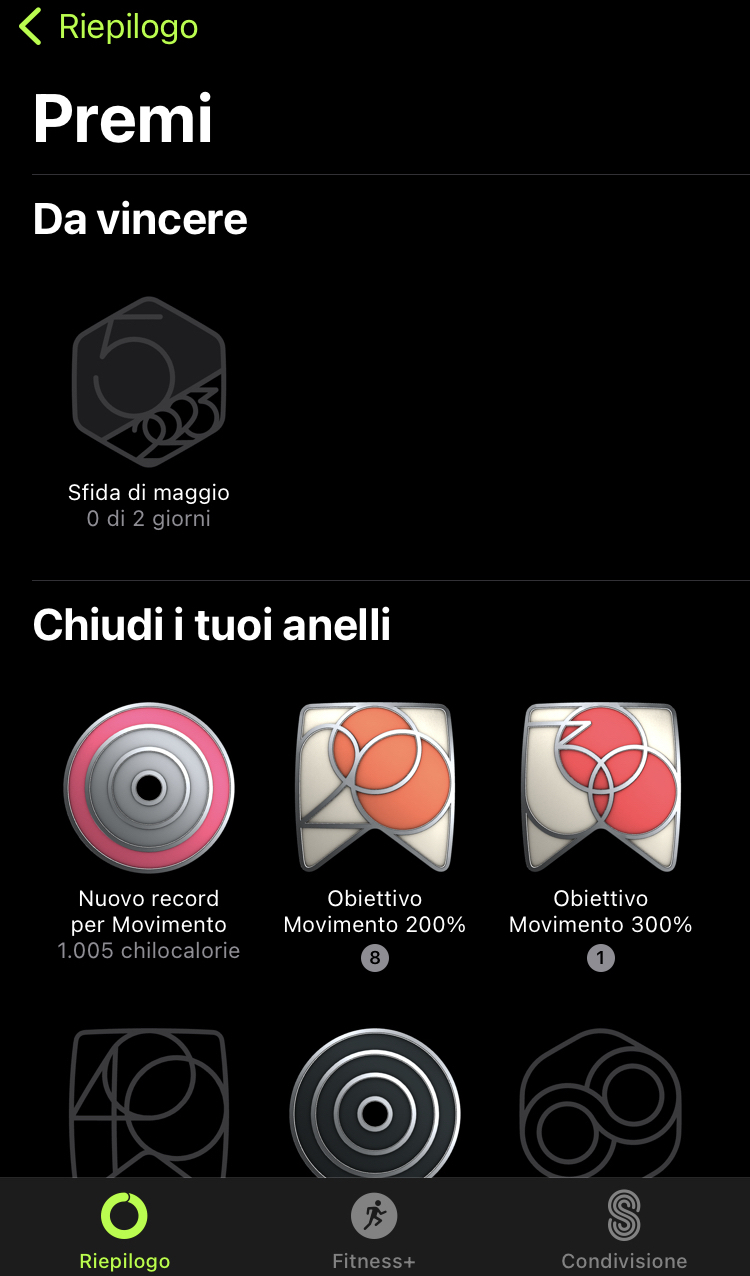
\includegraphics[width=0.4\textwidth]{img/apple-fitness-badge.jpeg}
        \label{fig:appleFitnessBadges}
    }
    \hspace{2em}% Space between image A and B
    \subfloat[Programma fedeltà Genius di Booking: sconti in base al livello]{
        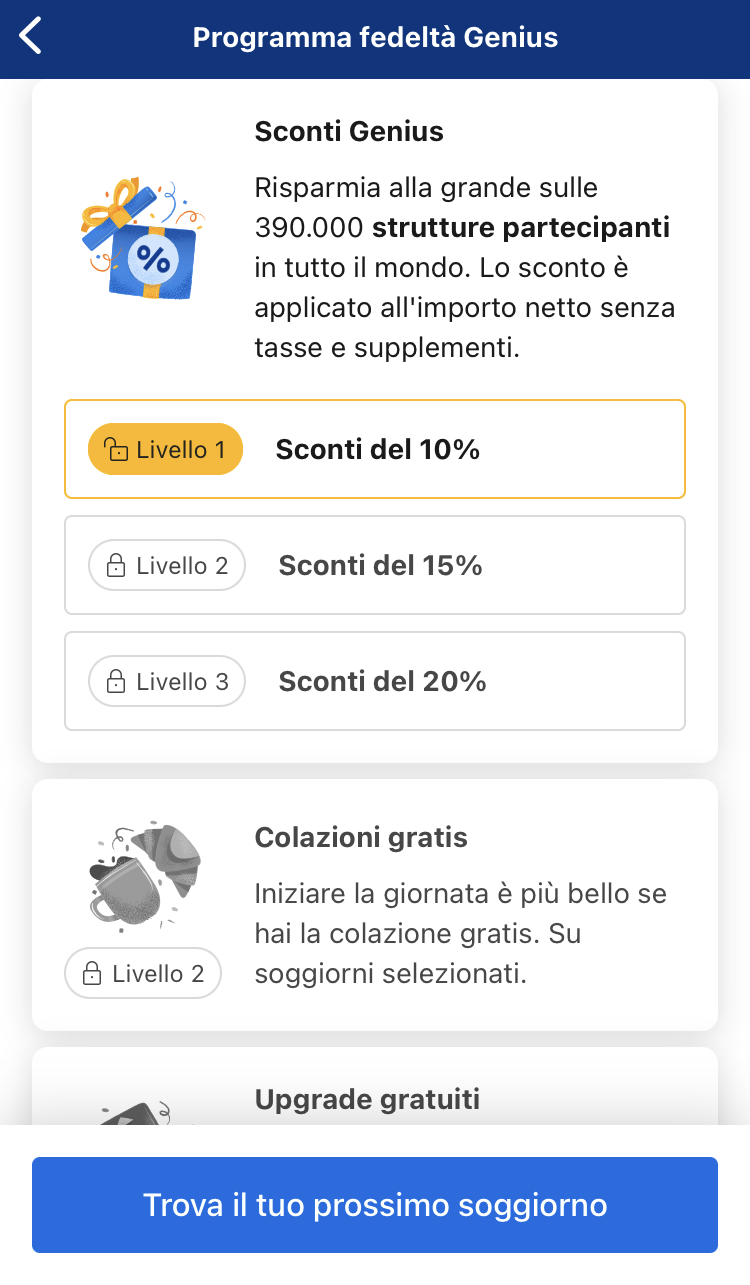
\includegraphics[width=0.4\textwidth]{img/booking-gamification.PNG}
        \label{fig:booking-genius}
    }
    \hspace{2em}% Space between image B and C
    \subfloat[App navigatore stradale Waze: tabellone punti e livello utente]{
        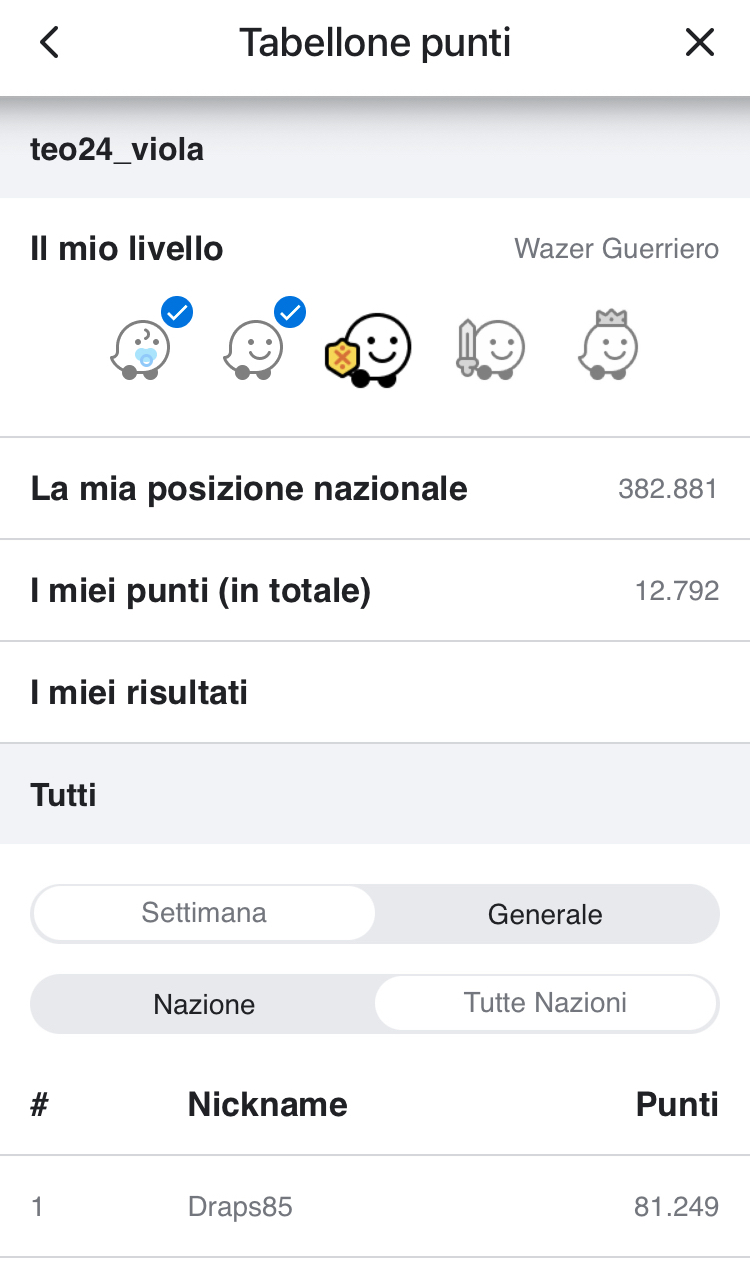
\includegraphics[width=0.4\textwidth]{img/waze2.jpeg}
        \label{fig:waze-level}
    }
    \caption{Esempi di piattaforme e app dove è presente la gamification} 
    \label{fig:gamification-example}
\end{figure}

\subsection{Serious game}
I Serious game, in italiano \enquote*{Giochi seri}, sono pensati e sviluppati con l'intento principale di educare, formare e successivamente d'intrattenere, in modo da rendere più piacevole, interessante ed efficace l'apprendimento; questi possono essere attività in cui si è fatto uso della gamification (\enquote*{Gameful design}) o veri e propri giochi, con o senza il supporto della tecnologia.

Nel caso vengano utilizzati supporti tecnologici si parla di \textit{Plugged Gamification} (es. Kahoot, Duolingo, \dots) altrimenti di \textit{Unplugged Gamification} (es. Quiz, puzzle, gare di teoria a squadre, \dots) \cite{pluggedGamificSeriousGame}.

\cite{seriousgame_langLearn}


% È stato dimostrato che questo genere di giochi possono migliorare l'attenzione e l'apprendimento se progettati correttamente;
% sono presenti studi che dimostrano che l'utilizzo di Serious Game aumenta l'efficacia dell'apprendimento da parte di studenti, e in alcuni casi anche grazie all'aiuto di tecnologie come la Realtà Estesa, Aumentata e Virtuale.
% Si cita uno dei tanti studi condotti per verificare l'efficacia di utilizzare la Realtà Estesa (AR, VR, MR) per insegnare in ambito medico ed effettuare simulazioni di operazioni chirurgiche dove è risultato che solo il 7\% dei casi non c'è stata maggiore efficacia nell'apprendimento \cite{HMDmedicalSeriousgame}, mentre nel resto degli altri casi c'è stata maggior motivazione, coinvolgimento ed efficacia da parte degli studenti.

%
\section{Extended Reality}
Extended Reality (XR), in italiano Realtà Estesa, è un termine che raggruppa tutte le possibili realtà che si possono generare utilizzando sistemi elettronici e informatici per portare una o più persone in realtà potenziate o totalmente generate dal computer.
Si identificano tre tipologie:

\begin{itemize}
    \item \textbf{Realtà Aumentata (AR)} L'ambiente reale circostante viene integrato con oggetti virtuali e/o informazioni utili aggiunti digitalmente;
    \item \textbf{Realtà Virtuale (VR)} La realtà circostante viene completamente sostituita con una virtuale;
    \item \textbf{Realtà Mista (MR)} \textcolor{red}{Il mondo reale e quello virtuale si mescolano.?}
\end{itemize}

\textcolor{red}{TODO: PARLARE DI COME SI PUò INTERAGIRE}

Nel caso degli Head-Mounted Devices (HMDs), grazie ai sensori e alle videocamere presenti, le interazioni possono avvenire usando il movimento della testa (Hand-free) oppure attraverso le proprie mani senza la necessita di dispositivi o strumenti specifici come puntatori, controller o guanti.

\subsection{Realtà aumentata}
La Realtà Aumentata (in inglese Augmented Reality, AR) consiste nell'arricchire il mondo reale circostante con oggetti e informazioni multimediali di vario genere e tipologia che normalmente non sarebbero percepibili dai cinque sensi.% Per alcuni si tratta di semplici sovrapposizioni d'informazioni attinenti al contesto in cui l'utente si trova mentre per altri affinché sia AR è necessaria una registrazione spaziale e/o una interazione con lo spazio circostante. \cite[ Capitolo 4, What is AR?]{whatMR}
Questi arricchimenti sono accessibili per mezzo di dispositivi come ad esempio visori AR, computer provvisti di webcam, smartphone, auricolari, lenti a contatto o tecniche particolari come il Video Mapping che fa uso di proiezioni sulle superfici e oggetti senza la necessità d'indossare alcun dispositivo (Spatially Argumented Reality\cite{Raskar1999SpatiallyAR}).

Si identificano tre tipologie di AR che si differenziano in base al criterio utilizzato per il posizionamento degli elementi \enquote{aumentanti} nell'ambiente circostante; si hanno quindi Realtà Aumentate:

\begin{description}
    \item \textbf{Location-based} (Figura \ref{fig:location_ar}) dove gli elementi vengono disposti in una precisa posizione geografica GPS, ad esempio viene mostrata una icona in corrispondenza di punti d'interesse (POI) in tempo reale, o viene emesso un suono specifico in corrispondenza di uno di questi;
    \item \textbf{Marker-based} (Figura \ref{fig:marker_ar}), gli oggetti vengono sovrapposti e posizionati sul marker che può essere un codice QR, una immagine o un disegno;
    \item \textbf{Markerless} (Figura \ref{fig:markerless_ar}), dopo una scansione dell'ambiente circostante, ad esempio con la fotocamera dello smartphone, gli oggetti vengono collocati su quelle caratteristiche ambientali ritenute adatte (es. Superfici orizzontali o verticali).
\end{description}

\begin{figure} [h]
    \centering
    \subfloat[Funzionalità Live View in Google Maps che utilizza l'AR Location-based]{
        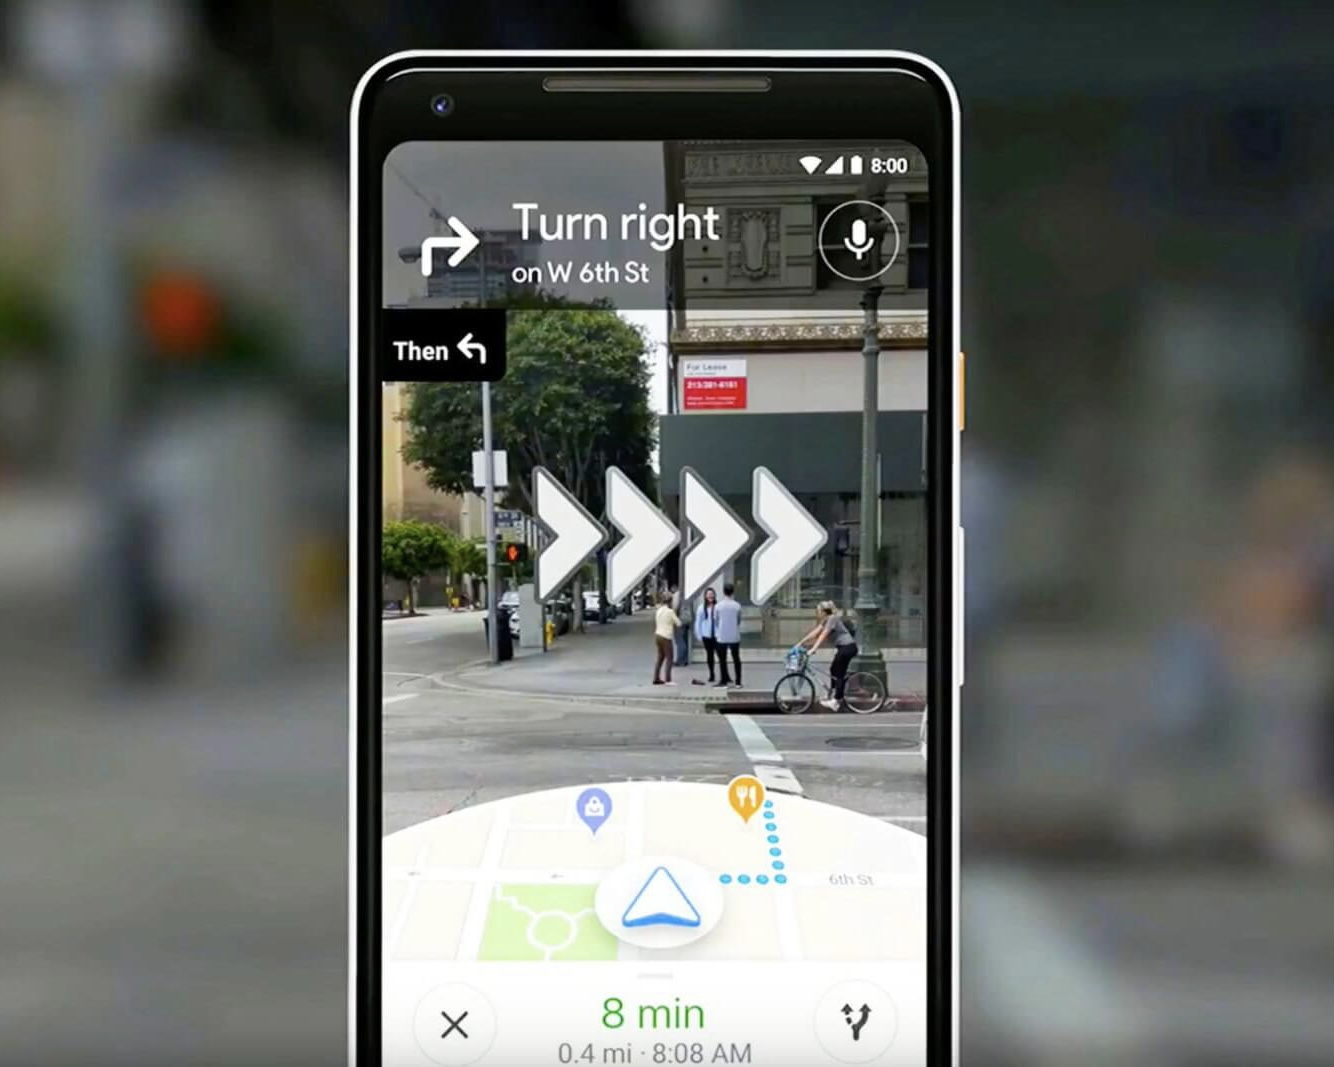
\includegraphics[width=0.32\textwidth]{img/location-based-ar.jpg}
        \label{fig:location_ar}
    }
    \subfloat[Marker-based AR]{
        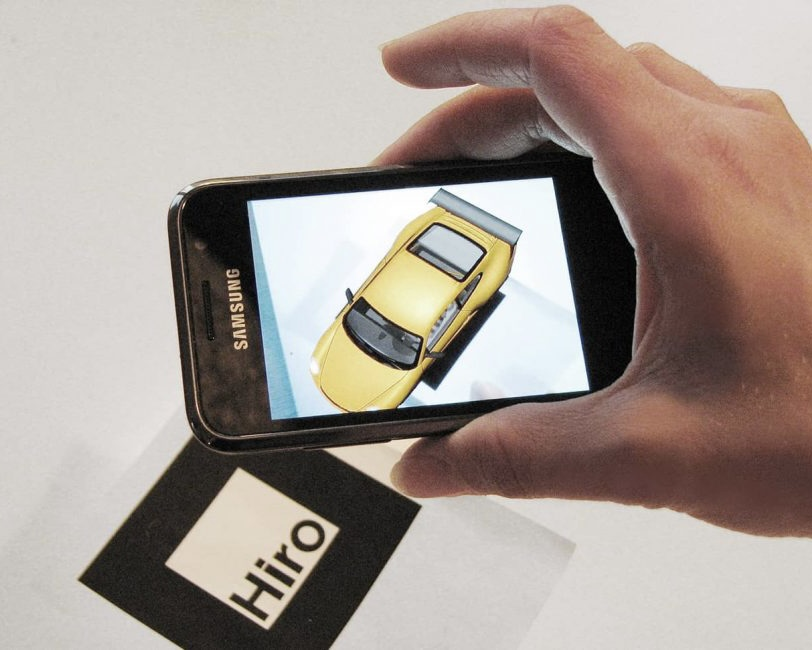
\includegraphics[width=0.32\textwidth]{img/marker-base-ar.jpg}
        \label{fig:marker_ar}
    }
    \subfloat[Markerless AR: App IKEA Place]{
        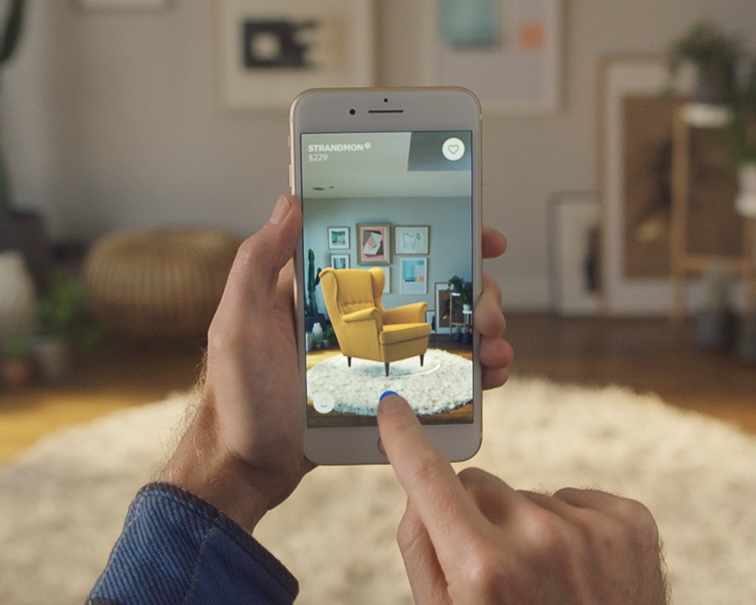
\includegraphics[width=0.32\textwidth]{img/markerless-ar.jpg}
        \label{fig:markerless_ar}
    }
    \caption{Esempi di tre tipologie di Realtà Aumentata} 
    \label{fig:ARbased_type}
\end{figure}

%% in Boschetto AR, al momento, non è possibile alcuna interazione con gli oggetti mostrati.

\subsection{Realtà virtuale}
La Realtà Virtuale (in inglese Virtual Reality, VR) sostituisce l'ambiente circostante con uno che realmente esiste (es. simulazioni) o completamente virtuale (es. videogiochi), isolando l'utente da tutte le interazioni sociali esterne. Questo genere di realtà sono necessari dispositivi hardware indossabili specifici come gli head mounted displays (HMD)\dots

\subsection{Mixed reality}

%
\section{Integrazione tra diversi tipi di device}
\section{Integrazione tra totem e smartphone}
    % ! TeX root = ../../main.tex
\chapter{Design e tecnologie}
\section{Requisiti}
% In  questo contesto il contributo di questa tesi mira ad aumentare l'interesse e la consapevolezza sul tema della ecosostenibilità e sul risparmio di carta attraverso l'integrazione di una applicazione per smartphone e un totem multimediale con anche l'aiuto della realtà aumentata e la \textit{gamification}.
Questa tesi ha l'obiettivo di sviluppare l'applicativo per un totem multimediale che si integri con l'applicazione mobile per smartphone BoschettoAR facente parte del progetto ReMade.
Nello specifico devono essere presenti diverse schermate che mostrano i progressi del progetto ReMade e i dati condivisi degli utenti.
%
\subsection{Requisiti funzionali}
Più precisamente devono essere presenti le schermate Home, statistiche, Classifica e Informazioni.
%TODO: scrivili in punto elenco e controlla se sono funzionali
La schermata principale chiamata \enquote{Home} deve mostrare un bosco ricco di alberi visto dall'alto (si vedono solo le chiome). Al tocco di un albero vengono mostrati i  (nickname,\dots) e le statistiche (contatori badge,...) relative all'utente corrispondente. Gli alberi devono cambiare la loro rappresentazione in base al livello raggiunto dall'utente.

La schermata delle Statistiche invece deve mostrare diversi contatori provvisti di un'icona rappresentativa, di una \textit{label} (etichetta) che specifica a cosa si riferisce il dato mostrato e infine il valore con unità di misura. Ciascun contatore al tocco deve mostrare una breve descrizione che spieghi il significato del valore.

La penultima pagina, quella della classifica, deve mostrare una classifica dei 10 migliori utenti sulla base della co2 risparmiata.
Gli elementi della classifica devono avere la posizione, il nickname dell'utente, la rappresentazione del livello dell'utente e quanta co2 hanno risparmiato.

La pagina delle Informazioni, deve mostrare diverse informazioni quali i calcoli fatti per ricavare i dati nella pagina delle statistiche e dettagli sul progetto a cui fa parte. Questa schermata deve essere il quanto più semplice possibile e può prevedere altre sezioni in caso di ulteriori informazioni da mostrare.

Oltre alle diverse pagine, deve essere presente una sezione o schermata sempre accessibile e visibile che permetta di avviare la modalità di caricamento dei dati utente dall'app al totem indistintamente dalla schermata visualizzata. Avviata la modalità deve essere visualizzato il qrcode identificativo del totem che verrà scansionato dall'app mobile.
%
\subsection{Requisiti non funzionali}
\begin{itemize}
    \item Il sistema deve essere scalabile in modo da permettere l'aggiunta di nuovi totem interattivi e gestire simultaneamente più richieste di condivisione dei dati dall'applicazione.
    \item L'interfaccia deve apparire familiare ed intuitiva, in modo da permettere un utilizzo immediato e non scoraggiare gli utenti all'interazione.
    \item La sincronizzazione dei dati deve essere, per quanto possibile, immediata in modo da mostrare sempre dati aggiornati.
\end{itemize}
%
%
%
\section{Design e mockup}
Prima di analizzare le scelte di \textit{design} e di mostrare i diversi \textit{mockup} sviluppati si introducono i significati delle due parole in corsivo utilizzate.

\begin{description}
    \item[Design] Il \textit{design} viene definito dal Cambridge Dictionary \cite{cambridgeDict} come \enquote*{il modo in cui qualcosa viene progettato e costruito o modellato} attraverso la stesura di un progetto che coniughi funzionalità ed estetica. Il \textit{design} può assumere diverse forme e fra queste ritroviamo anche il \textit{web design}, il \textit{graphic design} e l'\textit{interaction design}.
    \item[Mockup] Il termine \textit{mockup} o \textit{mock-up}, in italiano \enquote*{modello}, è una realizzazione a scopo illustrativo o espositivo di un oggetto o sistema, senza le complete funzioni dell'originale. Viene tipicamente sviluppato per fornire un'idea visiva del prodotto finale ai clienti, permettendo di effettuare correzioni o modifiche sulla bozza del prodotto ancora prima che si passi alla fase di sviluppo. Molti settori fanno uso di \textit{mockup} dal marketing alla editoria fino all'ingegneria. Nel settore del \textit{web design}, ad esempio, viene utilizzato per abbozzare il \textit{layout} di una pagina web e decidere la disposizione degli elementi, i colori, i caratteri del testo e le funzionalità interattive.
\end{description}

Per lo sviluppo del design grafico e del \textit{mockup} sono disponibili in commercio diversi programmi come Adobe XD, Balsamiq e Figma che è stato utilizzato in questo progetto.

La struttura principale dell'applicativo del totem si suddivide in due sezioni principali: la barra di navigazione e la pagina selezionata (figura \ref{fig:viewStruct}).
Nello specifico viene utilizzata la \textit{Navigation Rail} di Material Design come barra di navigazione verticale con l'inserimento in fondo di una sezione dedicata usata per la condivisione dei dati tramite app.

\begin{figure} [h]
    \centering
    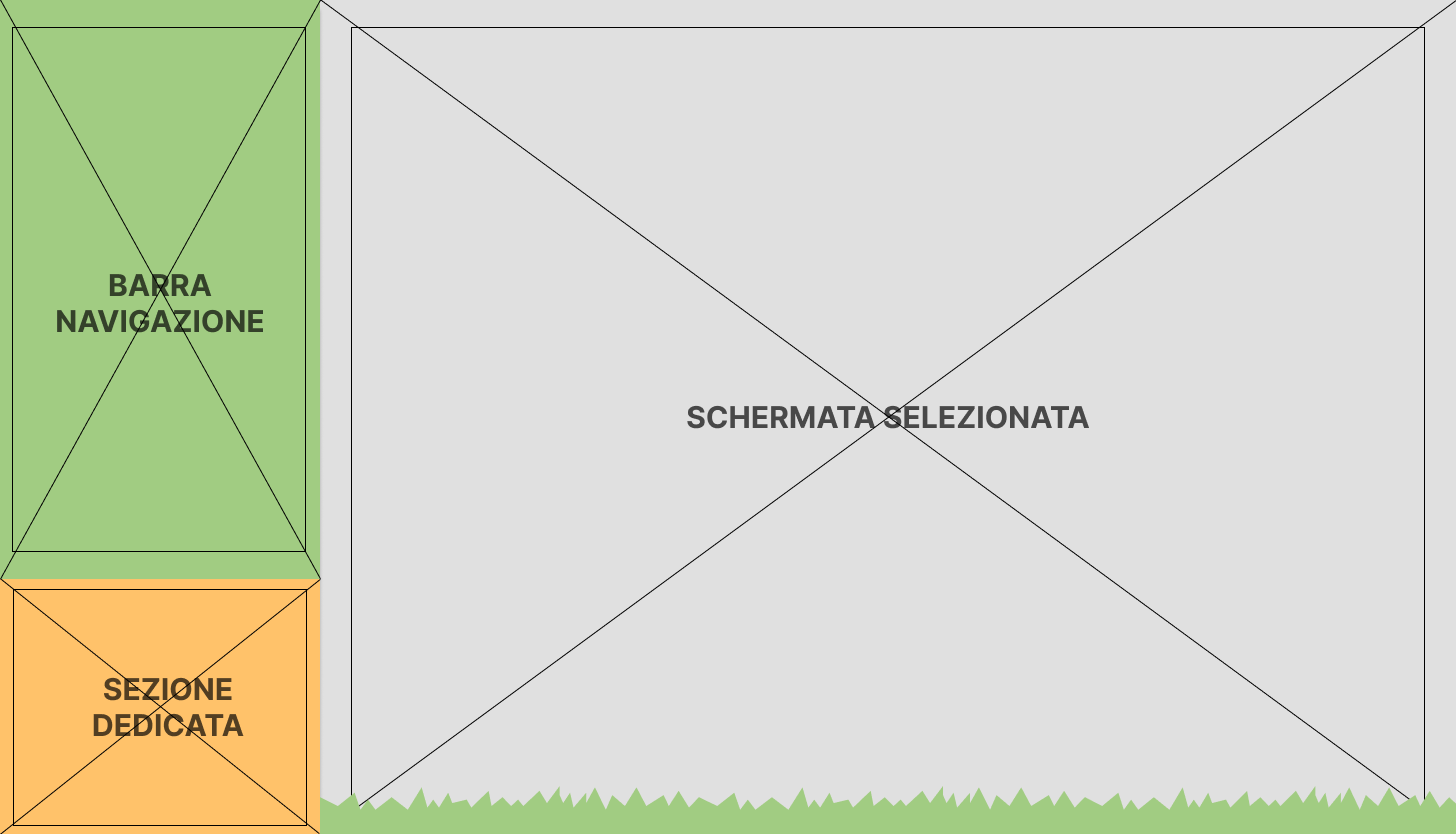
\includegraphics[width=0.8\textwidth]{img/mainStructure.png}
    \caption{Layout generale dell'applicativo del totem composto da tre blocchi: barra di navigazione (in verde), sezione dedicata (in arancione) e schermata selezionata (in grigio)}
    \label{fig:viewStruct}
\end{figure}

\subsection{Scansione codice QR totem}
In fondo alla barra di navigazione verticale si è posizionato il codice QR che identifica il totem per la condivisione dei progressi dell'utente tramite app.
In figura \ref{fig:depositIconsQR} viene mostrata l'icona del pulsante. Si compone di due immagini: un vaso ed una freccia verde (figura \ref{fig:hideQR}). Al tocco del pulsante la freccia svanisce, il vaso si ingrandisce fino a contenere al suo interno il codice QR (figura \ref{fig:showQR}).

\begin{figure} [h]
    \centering
    \subfloat[Codice QR del totem nascosto]{
        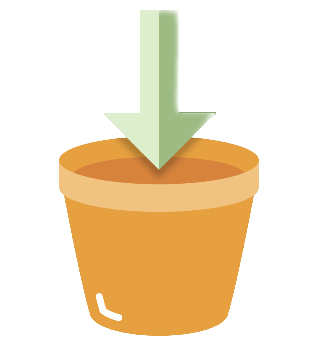
\includegraphics[width=4cm]{img/depositIcon.png}
        \label{fig:hideQR}
    }
    \vspace{1cm}
    \subfloat[Codice QR del totem visibile]{
        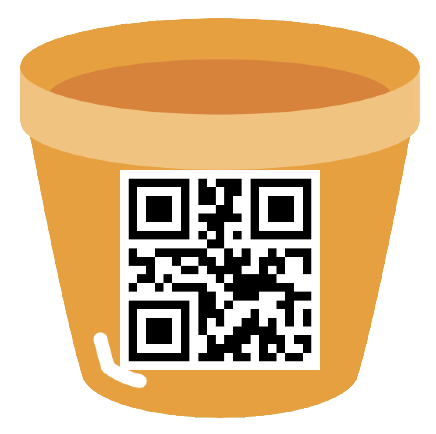
\includegraphics[width=4cm]{img/depositQR.png}
        \label{fig:showQR}
    }
    \caption{Pulsante per mostrare e nascondere il codice QR identificativo del totem per la condivisione dei dati da APP}
    \label{fig:depositIconsQR}
\end{figure}
%
\subsection{Homepage}
Per la \textit{homepage} sono stati pensati due design alternativi: uno mette in risalto gli utenti mentre l'altro fornisce una visione più globale della partecipazione degli utenti.
Il primo è organizzato in mensole su cui poggiano i vasi contenenti l'alberello che rappresenta il livello dell'utente (figura \ref{fig:shelfHome}). Più alto è il livello raggiunto più rigogliosa e prospera sarà la chioma. Le mensole sono disposte in modo da occupare lo spazio a disposizione. Questa soluzione riduce molto la quantità di utenti visualizzabili per volta, costringendo ad una paginazione delle mensole navigabile con frecce o pulsanti per cambiare pagina (questo dettaglio nel mockup non è stato inserito).
La seconda alternativa di \textit{homepage} invece permette di visualizzare molti più elementi rispetto alla precedente. La visualizzazione cambia prospettiva, viene abbandonata l'idea delle mensole e vengono mostrate le chiome degli alberi in visione aerea come se si guardasse un bosco dall'alto(figura \ref{fig:forestHome}).

\begin{figure} [h]
    \centering
    \subfloat[Visualizzazione a mensole]{
        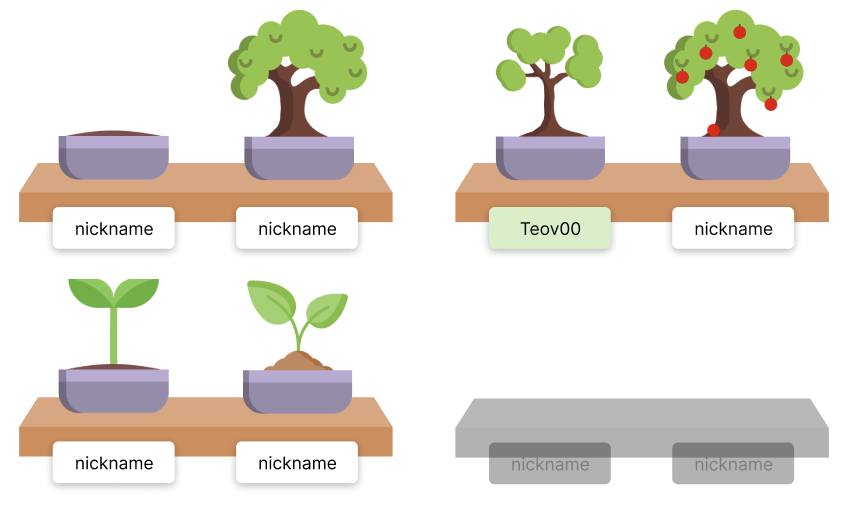
\includegraphics[width=0.45\textwidth]{img/shelfViewHome.png}
        \label{fig:shelfHome}
    }
    \subfloat[Visualizzazione a bosco]{
        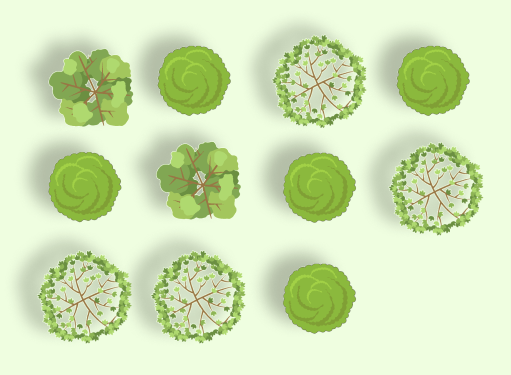
\includegraphics[width=0.45\textwidth]{img/forestViewHome.png}
        \label{fig:forestHome}
    }
    \caption{Possibili design di visualizzazione degli elementi della \textit{homepage}}
    \label{fig:homepages}
\end{figure}

In entrambe le alternative è presente un pannello che mostra i progressi dell'utente.

\subsubsection{Pannello dettagli utente}
Per il pannello dei dettagli sono state pensate tre diverse soluzioni: le prime due sono identiche se non per il particolare in basso (mensola e cordino, figure \ref{fig:shelfDetail} e \ref{fig:cordDetail}) mentre l'ultima si discosta completamente (figura \ref{fig:rectDetail}) sia graficamente sia per animazione.
\begin{figure} [h]
    \centering
    \subfloat[Stile mensola]{
        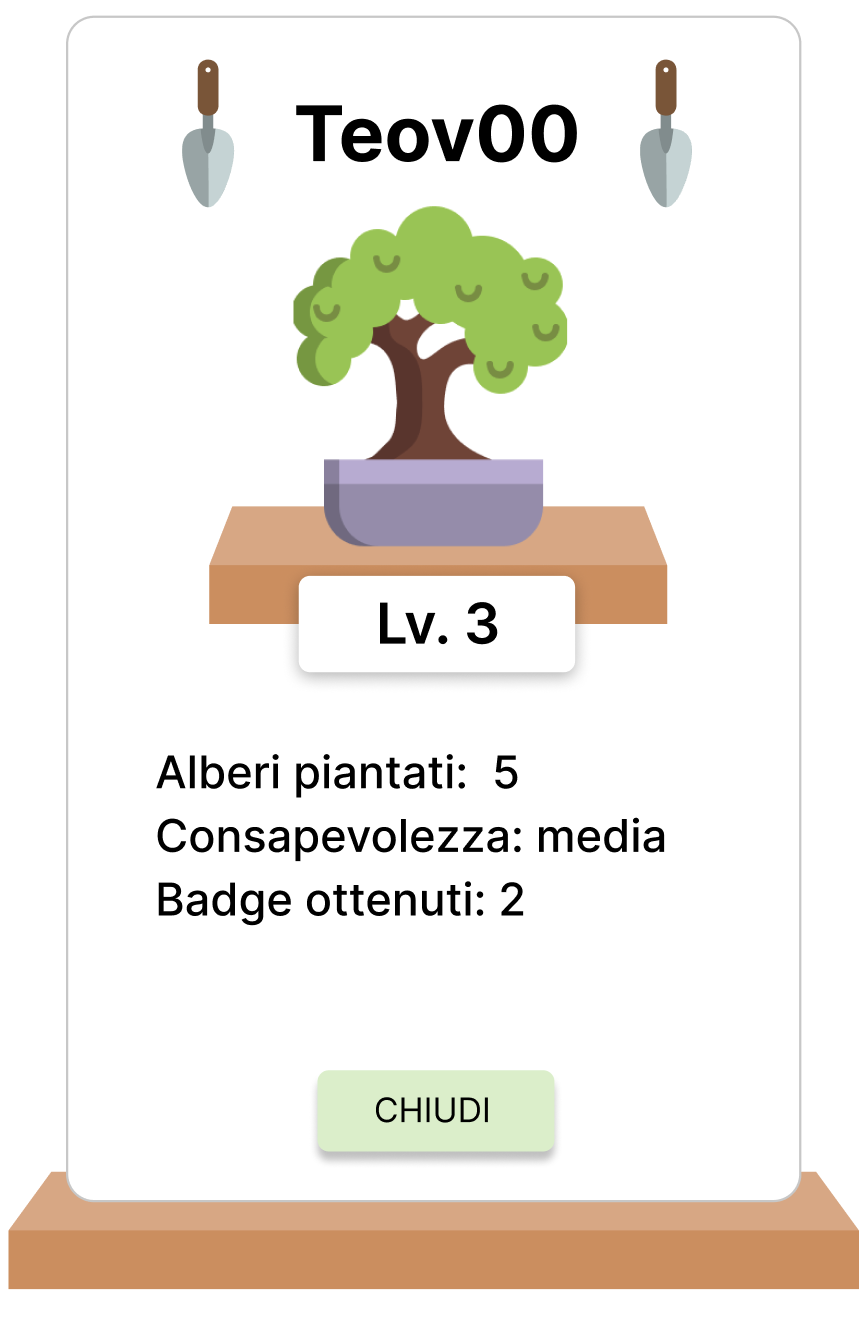
\includegraphics[width=0.33\textwidth]{img/shelfDetail.png}
        \label{fig:shelfDetail}
    }
    \subfloat[Stile tendina]{
        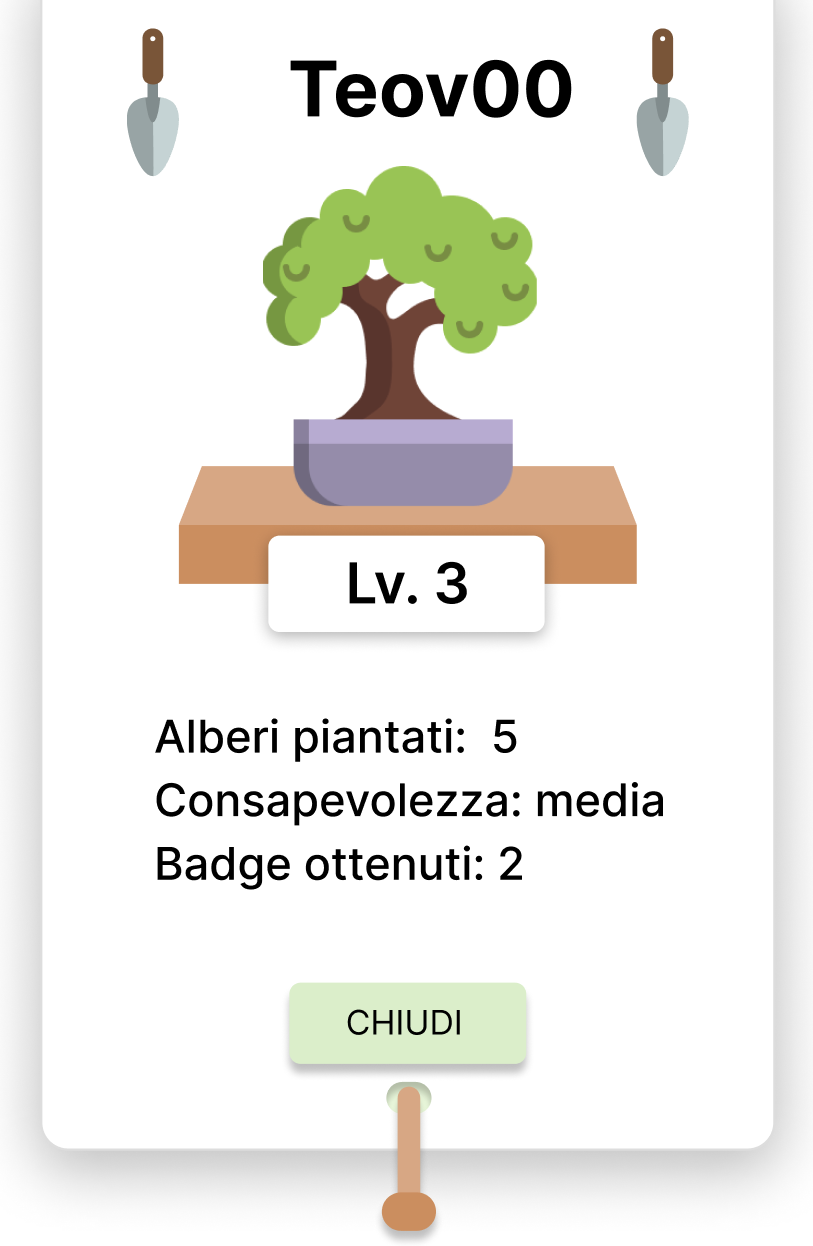
\includegraphics[width=0.32\textwidth]{img/cordDetail.png}
        \label{fig:cordDetail}
    }
    \subfloat[Stile rettangolo]{
        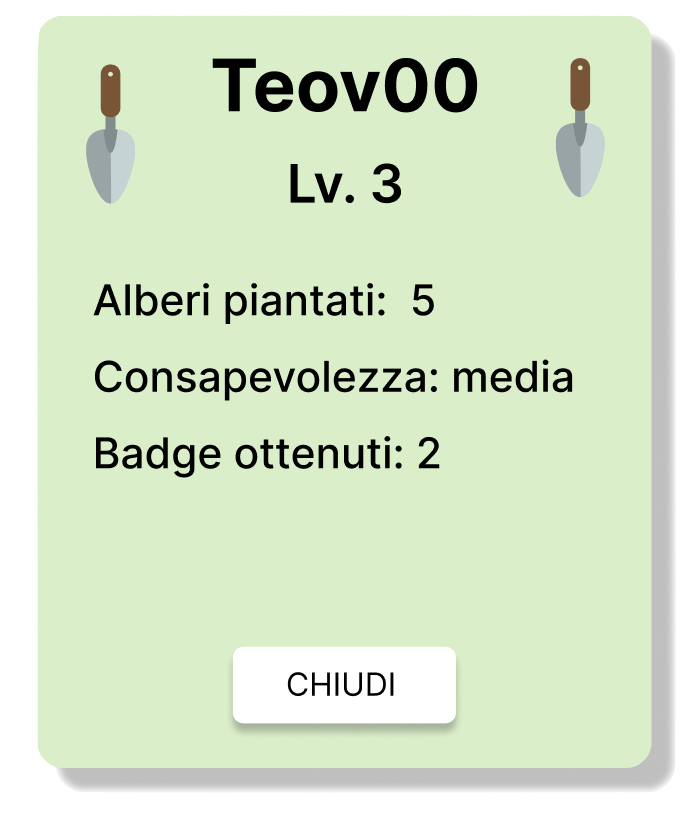
\includegraphics[width=0.33\textwidth]{img/rectDetail.png}
        \label{fig:rectDetail}
    }
    \caption{Tre diversi stili per il pannello dei dettagli: mensola, tendina e rettangolo}
    \label{fig:detailBanner}
\end{figure}
%
\subsection{Pagina statistiche}
La pagina delle statistiche presenta una disposizione a griglia con sei elementi, chiamati contatori, uno per ogni dato statistico (figura \ref{fig:statsPage}). Al tocco di un contatore questo si deforma diventando un quadrato e mostrando una breve descrizione del dato statistico al suo interno (figura \ref{fig:descrShowedStats}).

\begin{figure} [h]
    \centering
    \subfloat[]{
        
\includegraphics[width=0.3\textwidth]{img/plantedTreeStats.png}
        \label{fig:iconStats}
    }
    \subfloat[]{
        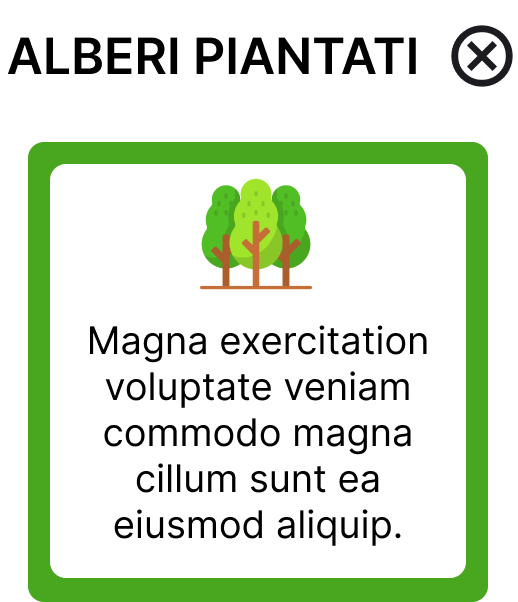
\includegraphics[width=0.3\textwidth]{img/plantedTreeStatsdescr.png}
        \label{fig:descrShowedStats}
    }
    \caption{Esempio di contatore nella pagina delle statistiche prima e dopo il tocco dell'utente}
    \label{fig:statCircle}
\end{figure}

\begin{figure}
    \centering
    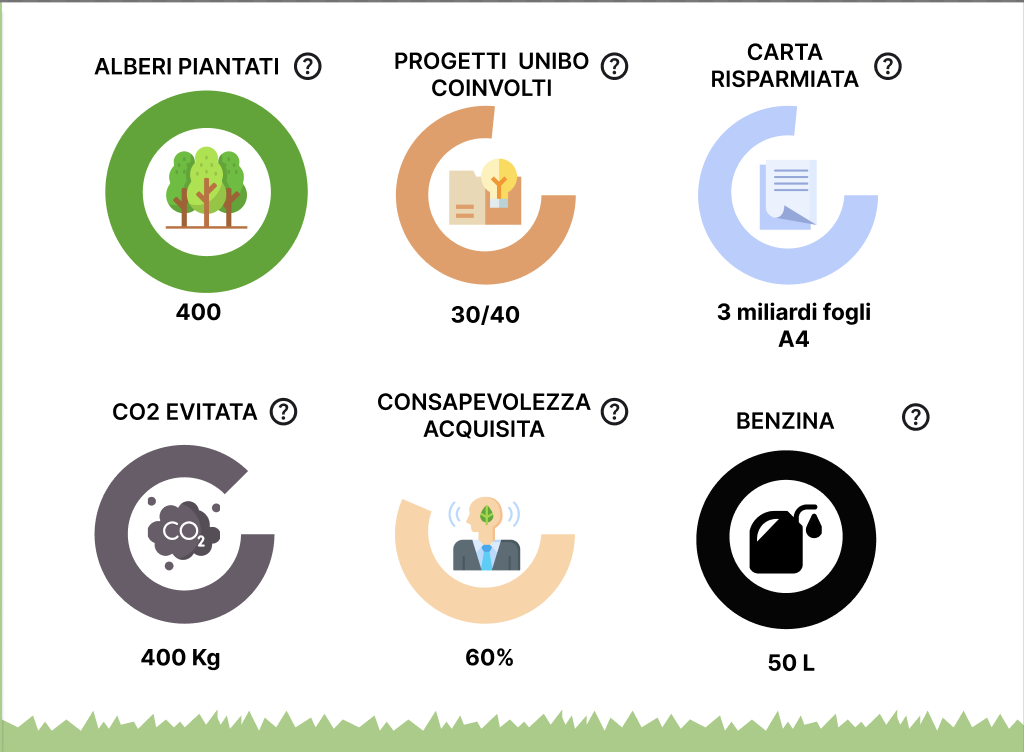
\includegraphics[width=0.8\textwidth]{img/statsPage.png}
    \caption{Mockup della schermata delle statistiche}
    \label{fig:statsPage}
\end{figure}
%
%
\subsection{Pagina della classifica}
%%TODO: write something
\begin{figure}
    \centering
    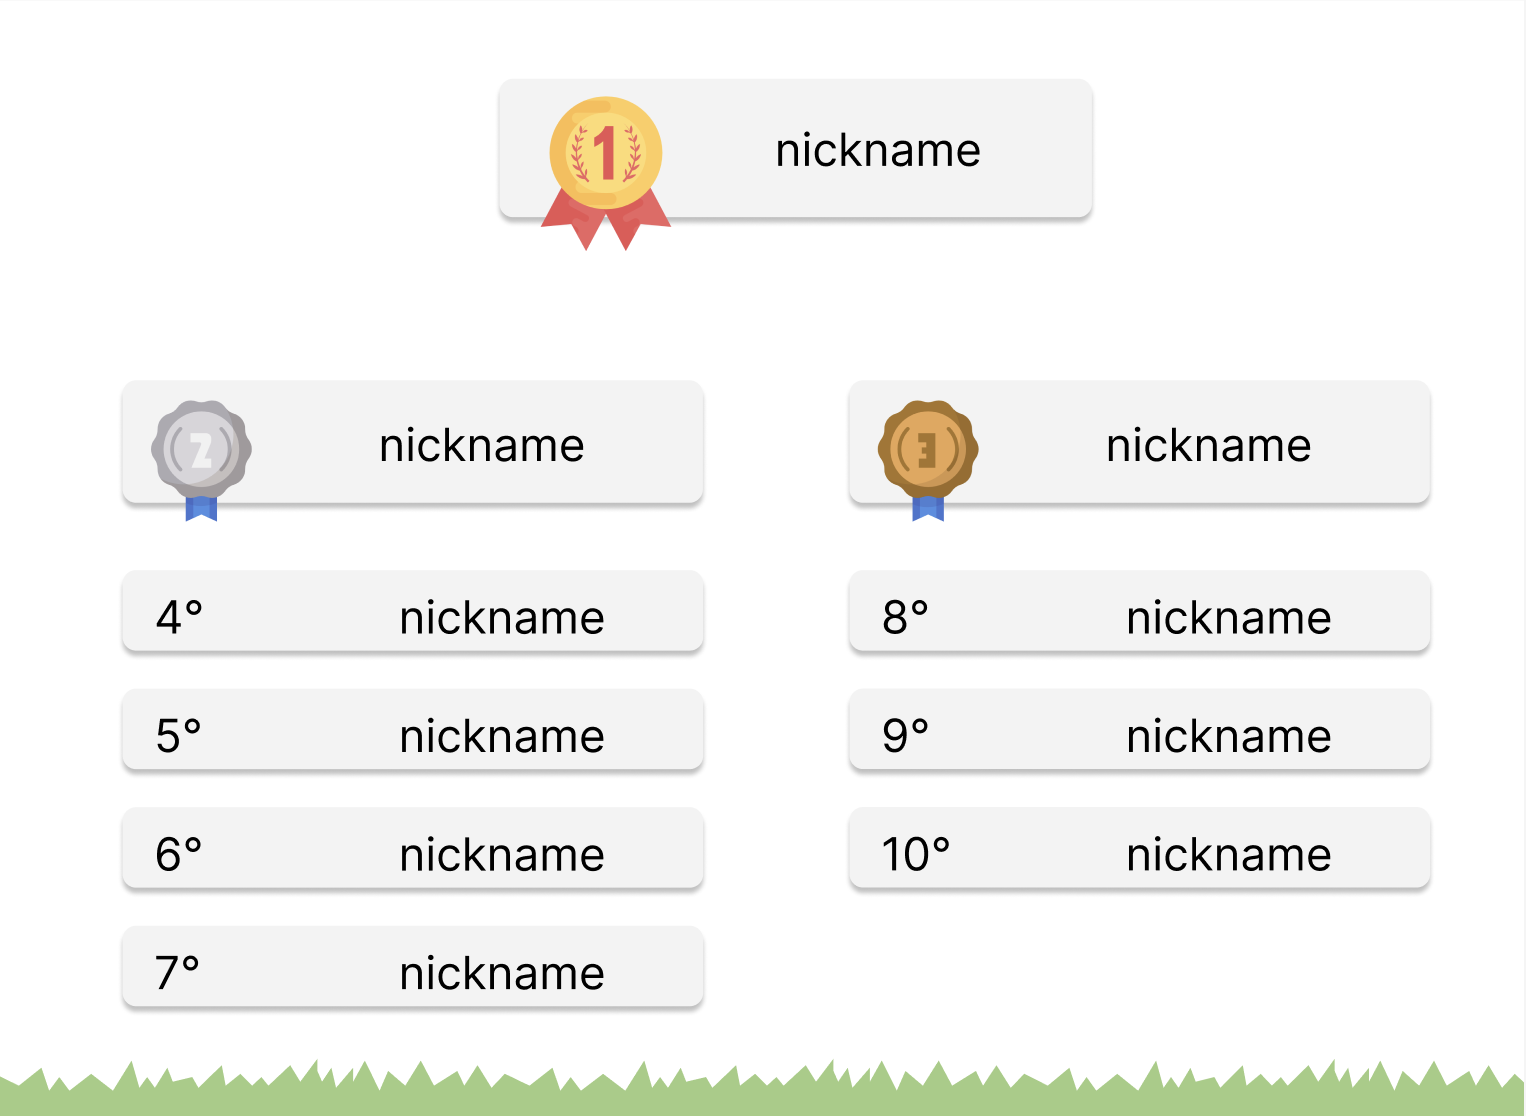
\includegraphics[width=0.8\textwidth]{img/topchartPage.png}
    \caption{Mockup della schermata della classifica}
    \label{fig:chartPage}
\end{figure}
%
\subsection{Pagina delle informazioni}
Questa pagina è stata pensata inizialmente come un'unica pagina scorribile verticalmente, simile ad una pagina web. Il tipo d'interazione con lo schermo, con questo \textit{design} e \textit{layout}, poteva risultare difficile e poco comoda considerata la grandezza dello schermo.
Si è optato quindi per un \textit{design} semplice con delle \enquote*{piastrelle} (dette \textit{tiles}) disposte a griglia. Con questo \textit{layout} è possibile avere le informazioni principali a colpo d'occhio e per ulteriori dettagli basta toccare la \textit{tile} interessata.

\begin{figure} [h]
    \centering
    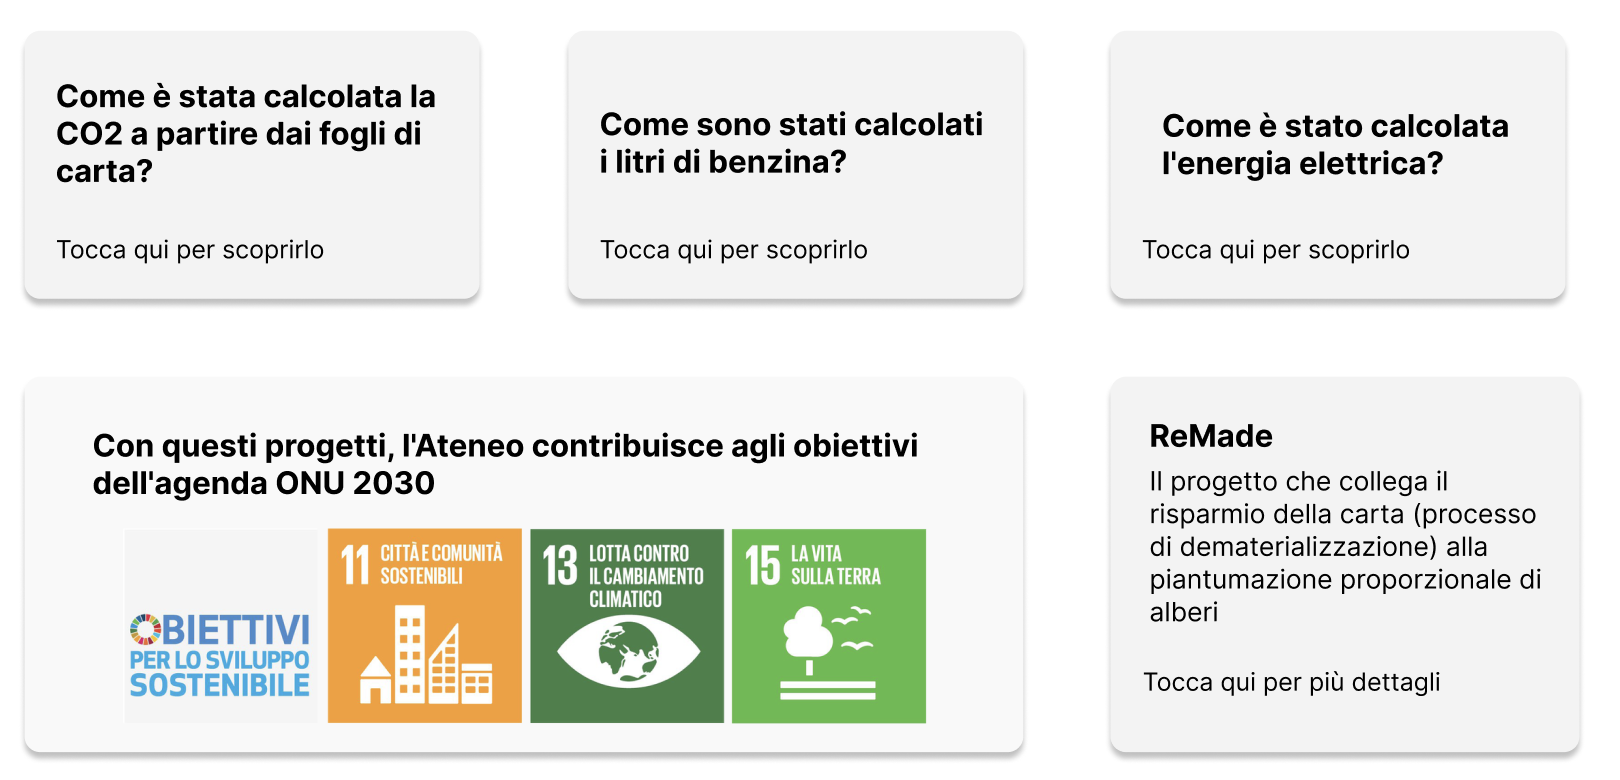
\includegraphics[width=0.8\textwidth]{img/infoPage.png}
    \caption{\textit{Mockup} della schermata delle informazioni}
    \label{fig:infoPage}
\end{figure}
%
%
%
\section{Tecnologie impiegate}
Di seguito vengono presentate le tecnologie utilizzate per lo sviluppo dell'applicativo del totem interattivo e della applicazione mobile. Per entrambi i dispositivi si è sviluppato utilizzando il framework Flutter, per l'integrazione e gestione dei dati è stato utilizzato il servizio cloud Firebase Realtime mentre per l'identificazione degli alberi e del totem sono stati utilizzati i codici QR.

\subsection{Applicazione Mobile}
Nel caso specifico dell'applicazione per smartphone sono state utilizzate la realtà aumentata (si rimanda al capitolo \ref{sec:ar}) e il database relazionale per la memorizzazione dei dati in locale.
% \subsubsection{Database Relazionale}
% per la memorizzazione dei dati in locale è stato creato e utilizzato un database relazionale opportunamente generato in base alla piattaforma di esecuzione dal \textit{plugin} di Flutter \texttt{sqflite}.

\subsection{Flutter}

%
\subsection{Firebase Realtime}
Firebase Realtime è un database non relazionale (NoSQL) memorizzato nel cloud. In quanto NoSQL, i dati e le relazioni non vengono memorizzati in tabelle ma in documenti, archivi \textit{wide-column} o grafi (nodi e archi) a seconda della tipologia del database.
Firebase Realtime è di tipo documentale e quindi fa uso di documenti simili ad oggetti JSON (\textit{JavaScript Object Notation}) per salvare i dati. Questo genere di memorizzazione permette maggiore flessibilità dello schema permettendo l'aggiunta o la modifica del modello dei dati. Inoltre i database NoSQL consentono una maggiore velocità e agilità di memorizzazione ed elaborazione oltre che offrire una maggiore scalabilità.

%
\subsection{Codici QR}
Il codice QR (\textit{Quick Response}) è un tipo di codice a barre a matrice (codice 2D) sviluppato e presentato nel 1994 dalla compagnia giapponese Denso Wave che si compone di tanti piccoli quadrati neri e bianchi, chiamati moduli, disposti in una matrice.
I codici QR permettono di memorizzare una quantità variabile di dati che dipende dalla tipologia di dato, dalla versione utilizzata e dal livello di correzione dell'errore. La dimensione della matrice è definita dalla versione utilizzata e anche dalla tipologia di codice QR (Modello 1/2, \textit{Micro QR Code}, \textit{rMQR Code}, \textit{SQRC} o Frame QR).

La versione più comune di \textit{QR code} è di tipo \textit{Model 1/2} di livello 3, presenta 29x29 moduli ed è in grado di memorizzare fino ad un massimo di 77 caratteri alfanumerici con la correzione dell'errore del 7\% circa.

%
% \subsection{Pagina Web Totem}
\section{Strumenti di sviluppo}
\subsection{Git}
Git è un \textit{Version Control System} VCS cioè un sistema di controllo delle versioni dei file. I cambiamenti di uno o più file nel tempo vengono memorizzati e questo permette di mantenere una cronologia dei cambiamenti e di ripristinare una versione precedente di file, cartelle o interi progetti. Esistono diverse tipologie di VCS: locale, centralizzato o distribuito.
Rispetto ai tradizionali VCS, Git non memorizza le differenze dei file (\textit{delta-based version control}) ma memorizza una istantanea di come appaiono i file nel \textit{filesystem} nell'istante in cui si effettua un salvataggio di versione (\textit{commit}). Git considera i suoi dati più come a un flusso d'istantanee del progetto che viene tracciato \cite{gitSite}.
%TODO: scrivere o elencare le caratteristiche utilizzate in git tipo il branching o che ne so
%
\subsection{Visual Studio Code}
Visual Studio Code è un editor di codice sorgente, sviluppato da Microsoft per Windows, Mac e Linux. Prevede diverse funzionalità utili per la scrittura di codice come la previsione e suggerimento di codice (IntelliSense) e gli strumenti di segnalazione e correzione degli errori, che i comuni editor di testo non possiedono.
Può essere utilizzato con la maggior parte dei linguaggi di programmazione (es. C, Java, PHP) ed è possibile aggiungerne di nuovi ed estendere le sue capacità attraverso dei \textit{plugin} scaricabili direttamente all'interno di Visual Studio Code.
Viste le qualità di questo editor e al suo utilizzo pregresso si è deciso di utilizzarlo per lo sviluppo di questo progetto con l'integrazione del \textit{plugin} ufficiale di Flutter che aggiunge ulteriori strumenti di analisi e \textit{debug}.
    % ! TeX root = ../../main.tex
\chapter{Implementazione}
In questo capitolo vengono trattate le implementazioni e i pattern utilizzati per raggiungere i requisiti di progettazione presentati nel capitolo precedente. Sono presentate le effettive schermate ottenute partendo dai mockup mostrandone porzioni di codice particolarmente interessanti o dove sono stati applicati pattern.

\section{Organizzazione progetto}
I file del progetto sorgente sono organizzati in cartelle relative a ciascuna schermata, componente o funzionalità. L'albero delle cartelle viene presentato nel listato \ref{lst:projectDir} dove vengono espanse solo le cartelle di primo livello (model, views e dataProvider). All'interno della cartella \texttt{model} sono state inserite le classi che definiscono il modello dei dati utente (file \texttt{share\_data\_model.dart}) e i metodi/classi/interfacce di utilità (file \texttt{obj2map.dart}), in \texttt{views} sono presenti i file delle schermate raccolti in cartelle e infine in \texttt{dataProvider} sono contenuti tutti i provider di dati utilizzati dal \texttt{DataManager} (file \texttt{data\_manager.dart}) per il reperimento delle informazioni.

\begin{lstlisting}[language=C, caption={Albero della directory del progetto TotemBoschettoAR}, label={lst:projectDir}]
    TotemBoschettoAR/
        |
        +- model/
            |
            +- obj2map.dart
            +- share_data_model.dart
        +- views/
            |
            +- common/
            +- navigation_menu/
            +- home_page/
            +- stats_page/
            +- chart_page/
            +- info_page/
            +- home_page.dart
            +- stats_page.dart
            +- chart_page.dart
            +- info_page.dart
        +- dataProvider/
            |
            +- firebase_provider.dart
        +- unit_converter.dart
        +- data_manager.dart
        +- main.dart
\end{lstlisting}

\section{App Mobile}
Seguendo i mockup sono state sviluppate le diverse schermate per la condivisione dei progressi. Sono state effettuate alcune modifiche come si può notare dagli screenshot in figura \ref{fig:shareDataApp}: in sostituzione al nickname utente impostato è stata messa una breve indicazione, che si trovava precedentemente nella pagina di scansione, sul come visualizzare il QR code del totem e infine la schermata di caricamento è stata modificata sostituendo l'icona e mostrando un testo che informi l'utente del caricamento dei dati.
\begin{figure}[h!]
    \centering
    \subfloat[Pagina di condivisone progressi]{
        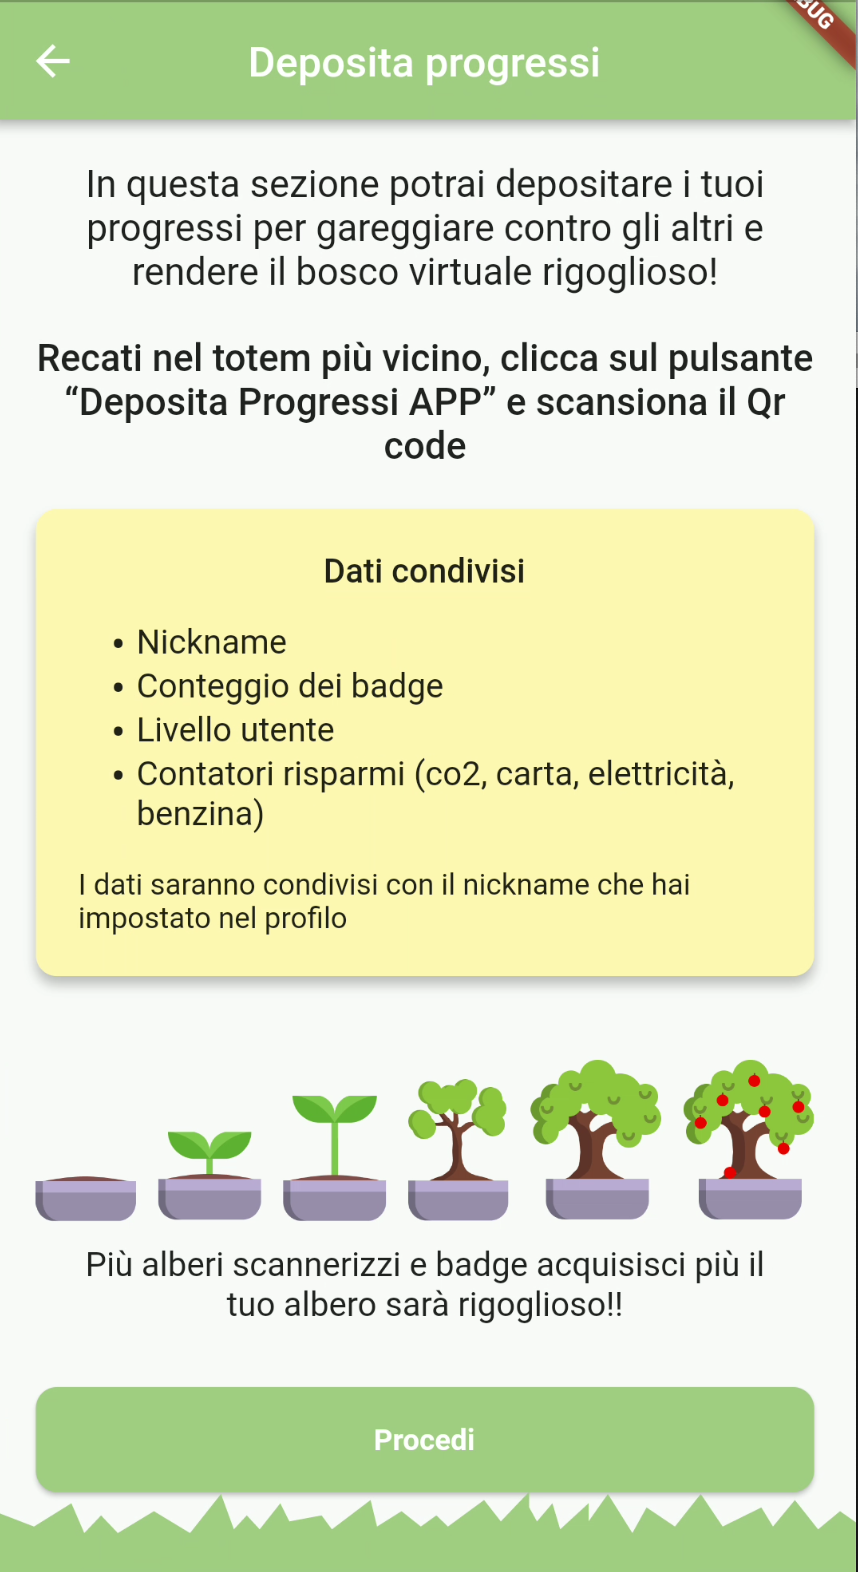
\includegraphics[width=0.3\textwidth]{img/app/uploadPage.png}
        \label{fig:sharePage}
    }
    \subfloat[Scansione QR code totem]{
        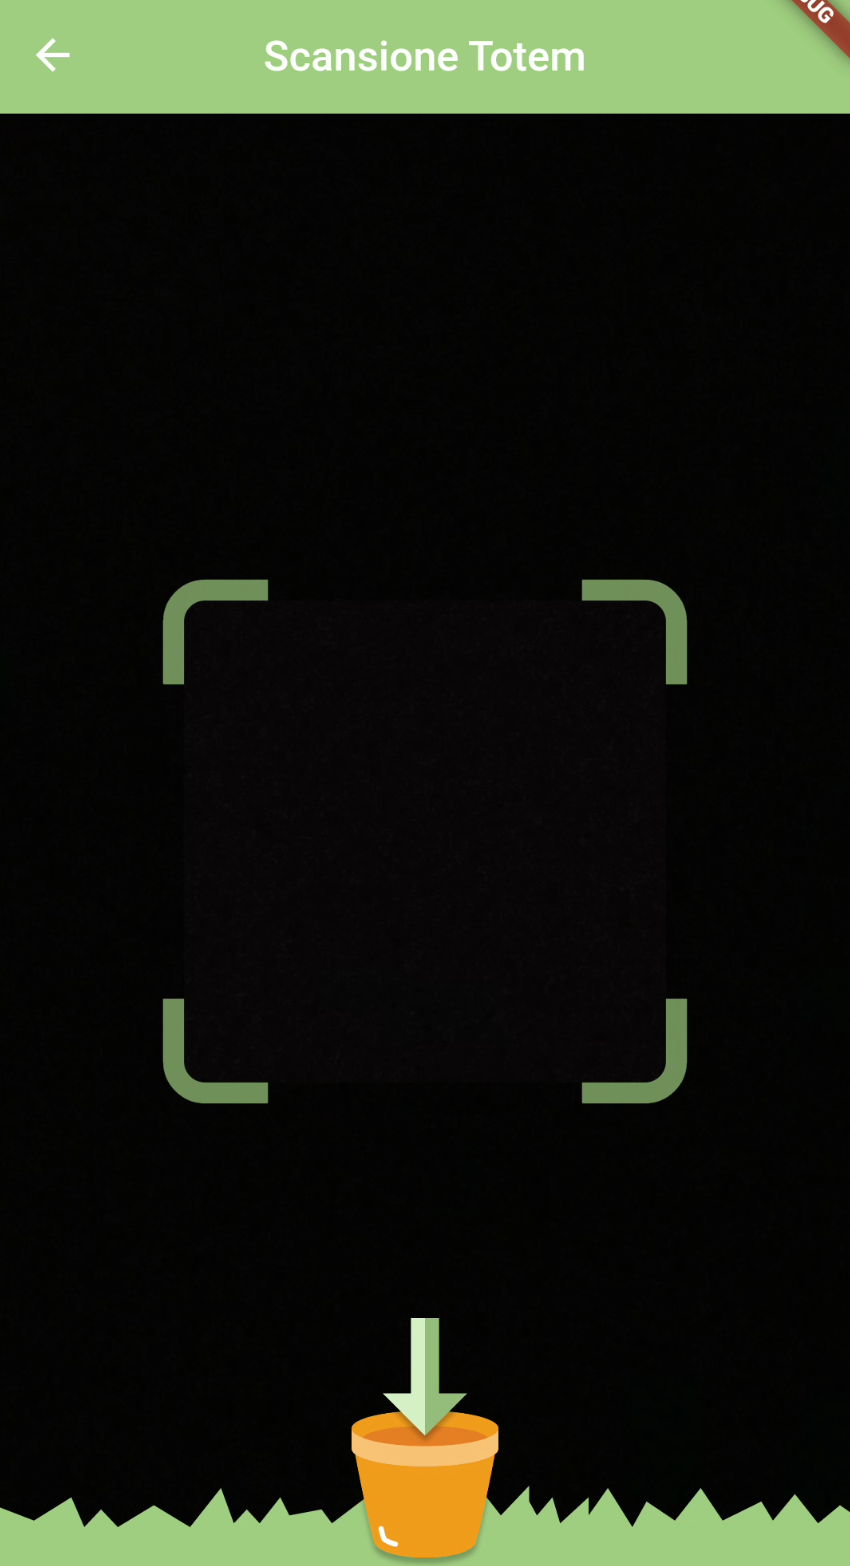
\includegraphics[width=0.3\textwidth]{img/app/uploadProgress.png}
        \label{fig:scanTotem}
    }
    \subfloat[Schermata di caricamento progressi]{
        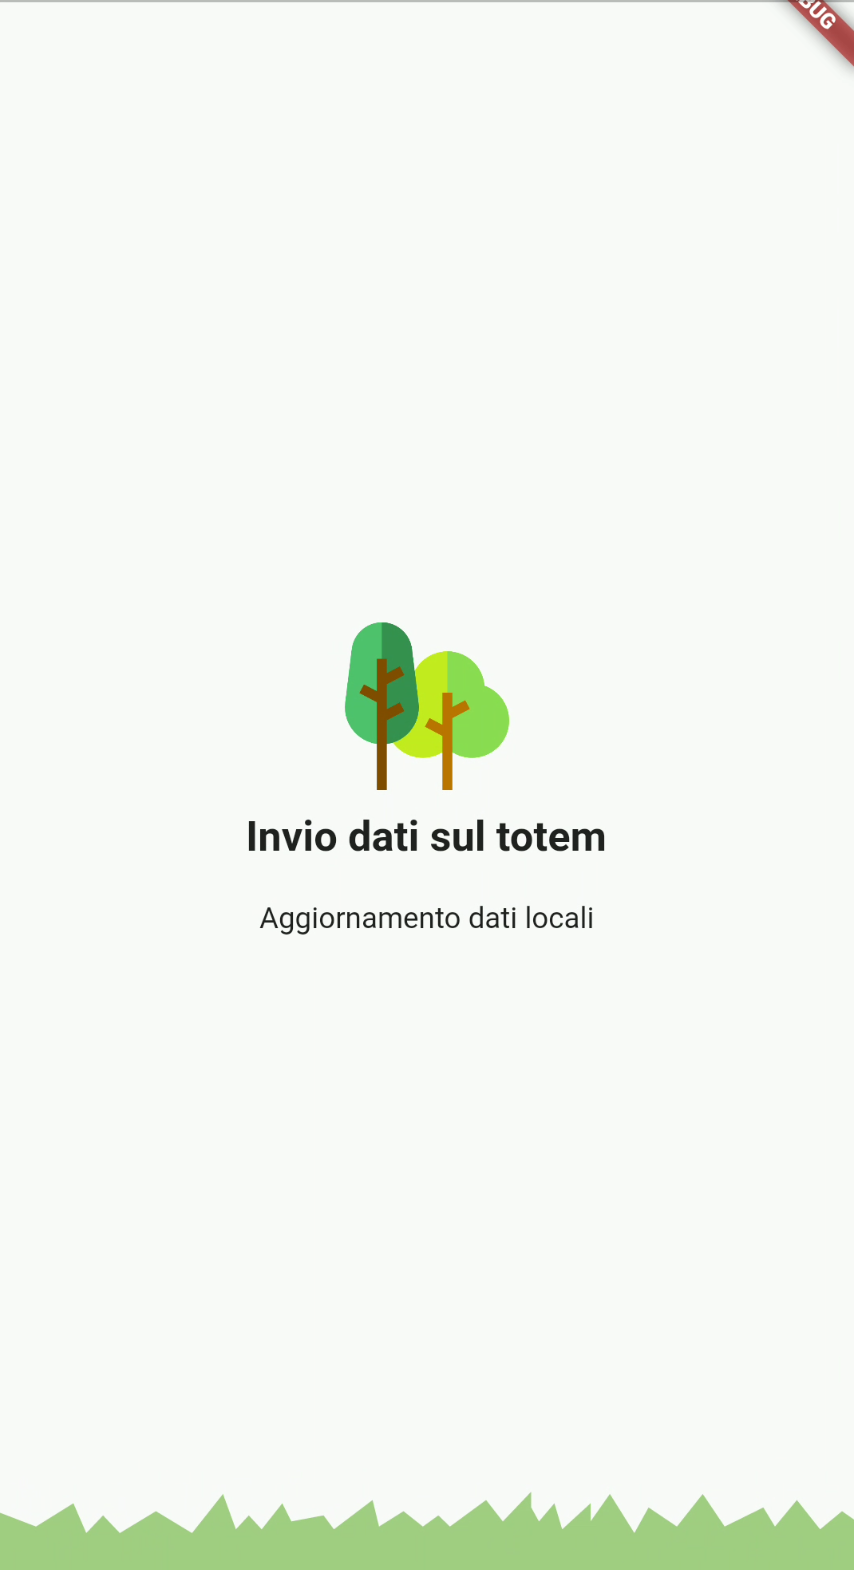
\includegraphics[width=0.3\textwidth]{img/app/uploadingPage.png}
        \label{fig:uploadinData}
    } 
    \caption{Screenshot schermate condivisione dati da app, scansione totem e caricamento}
    \label{fig:shareDataApp}
\end{figure}

\subsubsection{Pagina di condivisione progressi}
La schermata di caricamento dei progressi è raggiungibile dalla pagina utente oppure direttamente dalla pagina \textit{Home} in cui vi sono gli alberi collezionati. Nella barra degli strumenti (\texttt{AppBar}) di entrambe le pagine è stato aggiunto un pulsante (\texttt{IconButton})che permette di aprire la pagina di condivisione aggiungendola allo stack di schermate dell'app chiamando il metodo \textit{push} della classe \texttt{Navigator} che disciplina la navigazione fra pagine. Nel listato \ref{lst:shareIconButton} da riga 7 a riga 20 inclusa viene mostrato il codice inserito.

\begin{lstlisting}[style=FlutterStyle, caption={Codice aggiornato della barra degli strumenti dell'app: inserito pulsante per la condivisione dei progressi.}, label={lst:shareIconButton}]
    Scaffold (
      backgroundColor: Colors.white,
      appBar: AppBar(
        centerTitle: true,
        backgroundColor: mainColor, 
        title: const Text("Profilo"),
        leading: IconButton(
          onPressed: () => Navigator.push(
            context,
            MaterialPageRoute(builder: (context) {
              return const SharePorgressPage();
            }),
          ),
          icon: const Icon(
            Icons.upload,
            size: 25,
            semanticLabel: "Carica progressi",
          ),
        ),
      ),
      body: //contenuto della pagina Utente o della Home
    );
\end{lstlisting}

\subsubsection{Scansione QR e caricamento}
% Implementazione della schermata di scansione del qr del riutilizzo della schermata di scansione (forze pattern strategy), con schema d'interfaccia volendo 
% Implementazione della schermata con codice effettivo dell'implementazione del pattern mvi
\textcolor{red}{TODO: RIFORMULARE , IL CONCETTO è QUELLO}
La schermata della scansione del codice QR del totem prevede il riutilizzo della stesso componente utilizzato nella scansione del QR dell'albero. Infatti come si può vedere in figura ??, la schermata di scansione fa uso della classe \texttt{ScanQRView} che gestisce la fotocamera e la lettura dei codici QR. Riconosciuto un codice QR le informazioni contenute al suo interno vengono passate alla classe specifica per il totem che verifica la validità delle informazioni per poi procedere con la preparazione e caricamento dei progressi utente. Durante tutte le due fasi viene visualizzata la schermata in figura \ref{fig:uploadinData} che risulta reattiva in attesa di un esito del caricamento o della validità del codice QR.

Consiste specie di pattern strategy E in cui oltre la strategia che viene utilizzata per la validazione del codice QR scansionare si indica anche la schermata barra interfaccia utente che deve essere visualizzata dopo la scansione del codice. Ciò schermata poi possiede la sua strategia per validare ed utilizzare i dati presi dal QR.
\textcolor{red}{scegli se mettere solo future builder o tutta la classe}

 \begin{lstlisting}[style=FlutterStyle, caption={}, label={lst:strategyViewTotem}]
  Consumer<DataManager>(
    builder: (context, dataManager, child) => FutureBuilder<bool>(
      future: dataManager
          .uploadUserData(totemId)
          .timeout(const Duration(seconds: 8)),
      builder: (context, snap) {
        ConnectionState conState = snap.connectionState;
        bool uploadDone = snap.hasData ? snap.data! : false;
        if (conState == ConnectionState.waiting) {
          return const UploadingDataView();
        } else if (conState == ConnectionState.done) {
          if (uploadDone) {
            return const CompletedUploadView();
          } else {
            return const ErrorView(message: "Errore invio dati");
          }
        } else {
          return const ErrorView(message: "Errore sconosciuto");
        }
      },
    ),
  ),
\end{lstlisting}
%%%%%%%%%%%%%%%%%%%%% TOTEM %%%%%%%%%%%%%%%%%%%%%%%%%%%%%%%%
\section{Totem}
\subsection{Dati Firebase}
Una volta deciso di utilizzare il database Firebase Realtime, che è di tipo documentale, si è reso necessario convertire lo schema UML in figura \ref{fig:totemDomain} in formato JSON per avere la struttura generale dei dati che verranno memorizzati.
Per non avere troppi oggetti annidati, si è deciso di separare le informazioni del totem (listato \ref{lst:totemInfo}) dai dati utente che sono stati condivisi (listato \ref{lst:userDataTotem}).

\begin{lstlisting}[language=json, caption={Esempio di oggetto JSON contenente le informazioni sui totem}, label={lst:totemInfo}]
    "totemInfo": {
        "totemIdString": {
          "place": "locationName",
          "project": "projectName"
        },
      },
\end{lstlisting}  

\begin{lstlisting}[language=json, caption={Esempio di oggetto JSON che memorizza i dati utente per ciascun Totem}, label={lst:userDataTotem}]
      "totems": {
        "ces_remade": {
          "userNickname": {
            "badgeCount": 0,
            "co2": 0,
            "level": 0,
            "nickname": "userNickname",
            "paper": 0,
            "treesCount": 0
          }
        }
      }
\end{lstlisting}

\subsection{DataManager}
%Come è il datamanager, cosa ritorna e come viene gestito il pattern observer di Firebase che chiama metodo dopo che il db viene modificato
Il DataManager, come spiegato nel capitolo del design, funge sia da Repository che da Model del pattern MVI. Mantiene al suo interno i riferimenti ai diversi provider di cui fa uso, al momento solo \texttt{FirebaseProvider}, ed espone metodi che restituiscono \textit{State}, indirizzati alla \textit{View}, contenenti i dati utili alle schermate. A livello implementativo gli \textit{State} sono un oggetto della classe \texttt{Future} e vengono utilizzati come risultato ad una computazione asincrona permettendo di svolgerne altre finché non viene completata. Utilizzando \texttt{Future} come tipo di ritorno dei metodi del DataManager in combinazione con il \texttt{FutureBuilder} si individua una forma di pattern MVI con la possibilità di adattare la View in base allo stato della computazione.

La classe \texttt{DataManager}, come si può notare in riga 1 del listato \ref{lst:dataManager}, estende \texttt{ChangeNotifier} e questo permette d'informare la View della presenza di nuovi dati aggiornati.
Inoltre viene utilizzato il pattern Observer sul FirebaseProvider: il DataManager, implementando l'interfaccia \texttt{FirebaseObserver} e aggiungendosi come observer (riga 8 listato \ref{lst:dataManager}), viene notificato per qualsiasi genere di modifica dei dati nel cloud.
In cascata quindi ogni modifica sul database Firebase fa scattare la notifica delle Views con il metodo \texttt{notifyListeners} (riga 25 listato \ref{lst:dataManager}).

\begin{lstlisting}[style=FlutterStyle, caption={Classe DataManager}, label={lst:dataManager}]
  class DataManager extends ChangeNotifier implements FirebaseObserver {
    final String _totemId = "ces_remade";
    late final FirebaseProvider _firebaseProvider;
  
    DataManager() {
      _firebaseProvider = FirebaseProvider(_totemId);
      _firebaseProvider.addObserver(this);
    }
  
    String getCurrentTotemId() {
      return _totemId;
    }
  
    Future<List<SharedData>> getData() async {
      return _firebaseProvider.getTotemData();
    }
  
    Future<List<SharedData?>> getTop10User() async {...}
  
    Future<Map<StatId, String>> getStatistics() async {...}
  
    @override
    void firebaseNotify() {
      notifyListeners(); 
    }
  }
\end{lstlisting}

\subsection{Pagina Homepage}

\subsection{Pagina Statistiche}
Animazione dell'elemento della griglia, creazione della pagina, quali widget flutter sono stati utilizzati e codice di pattern mvi per il caricamento dei dati e la loro attesa, operazioni che vengono svolte all'interno di data manager per ricavare i dati

\subsection{Classifica}
Schermata della classifica, le modifiche grafiche che ha subito, l'aggiunta dell'alberello e info di co2, caricamento dati solito pattern mvi, come viene stilata la classifica codice lato repository (datamanager)... Ipotesi di poter decidere su cosa viene fatta la classifica es. co2, benzina o che altro. anche se poi alla fine le quantità sono proporzionali, cambierebbe poco la classifica.

\subsection{Pagina Informazioni}
Pagina informazioni, struttura a griglia, le classi che sono state create e politica di disposizione delle tiles;  pattern observer per mostrare e chiudere il pop up delle info
come si deve fare per aggiungere una tile e impostazioni delle tile, grandezza e contenuto


    \backmatter
    \chapter{Conclusioni}
%%------------- PARTE RIASSUNTIVA TESI -------------%%
% Nelle conclusioni, invece, si fa una prima parte molto riassuntiva del volume di tesi, per poi raccontare gli sviluppi futuri (di solito è più corto dell’introduzione). 
In questo elaborato si è descritto lo sviluppo dell'applicativo del totem e della sua integrazione con l'app mobile, utilizzando diverse tecnologie, partendo dalla fase di design architetturale e grafico, con l'aiuto di strumenti come schemi e mockup, fino ad arrivare alla fase d'implementazione in cui vengono spiegate nel dettaglio le implementazioni delle schermate del totem mostrandone il codice e gli screenshot del risultato finale.

Nella progettazione sono stati utilizzati elementi di gioco come i badge, i livelli e la classifica in modo da giovare dei vantaggi che porta la gamification e di tecnologie come il cloud computing per il salvataggio dei dati, i QR code e la Realtà Aumentata che permette di concretizzare, agli occhi degli utenti, i dati numerici che vengono mostrati sotto forma di oggetti virtuali (plichi di carta e taniche di benzina), migliorandone la comprensione.

In particolare integrando l'app BoschettoAR con il totem interattivo si è cercato di sensibilizzare ulteriormente gli utenti sul tema della dematerializzazione e della piantumazione di alberi e sul come sia possibile raggiungere grandi risultati ecologici, come la riduzione di CO\textsubscript{2}, attraverso la partecipazione e collaborazione e di tutti.

Grazie al totem, gli utenti sono in grado di tenere traccia dei loro progressi confrontandoli con quelli degli altri attraverso la classifica e la visualizzazione dei progressi raggiunti da ogni singolo utente, in una sorta di competizione, e di contribuire nella creazione di un bosco virtuale sempre più ricco e verde aumentando la consapevolezza della comunità universitaria.

%%------------- SVILUPPI FUTURI -------------%%
Nonostante siano stati raggiunti tutti gli obiettivi prefissati, definiti dai requisiti presentati nel secondo capitolo, è presente ancora un buon margine di miglioramento e ampliamento con nuove funzionalità.

Per poter migliorare e incrementare il coinvolgimento degli utenti occorrerebbe implementare una dinamica più stimolante dello sblocco dei badge e del passaggio al livello successivo, proponendo sfide o quiz periodici da superare, anche attraverso l'uso della Realtà Aumentata.

Sarebbe inoltre molto interessante diffondere questo progetto nelle altre sedi dell'Ateneo introducendo sfide ed eventi che le vedano coinvolte con la possibilità d'inserire anche nei totem il concetto dei badge.

Per impedire che gli utenti perdano i propri dati e progressi dell'app mobile si potrebbe offrire la possibilità di esportare i dati in un file o di permettere il salvataggio sul cloud il che porterebbe all'introduzione della creazione facoltativa di un account dell'utente.
    % ---------------------------------------------------------------------
    % Backmatter command leaves the page numbering alone but switches the 
    % chapters back to being not numbered.
    % ---------------------------------------------------------------------
    \nocite{*}{
        \printbibliography[
            heading=bibintoc,
            title={Bibliografia}
        ]
    }
    \chapter{Ringraziamenti}
\thispagestyle{empty}
Qui possiamo ringraziare il mondo intero!!!!!!!!!!\\
Ovviamente solo se uno vuole, non \`e obbligatorio.
    % ---------------------------------------------------------------------
    % Appendix
    % ---------------------------------------------------------------------
    \appendix
\end{document}